
\documentclass[12pt,a4paper]{article}

% =====================================================================
%  VITAICARE — wrapper de compilación
%  El CUERPO se escribe en tesis.md y se genera con  bash build.sh
%  -> produce cuerpo.tex, que este archivo incluye con \input.
%  Este archivo conserva el preámbulo y la portada de main.tex;
%  la única diferencia es la bibliografía: biblatex (IEEE) en vez de ieeetr.
% =====================================================================

% ---------- Idioma y codificación ----------
\usepackage[spanish, es-tabla]{babel}
\usepackage[T1]{fontenc}
\usepackage[utf8]{inputenc}   % (pdflatex)
\usepackage{lmodern}
\usepackage{microtype}

% ---------- Márgenes / espaciado ----------
\usepackage{geometry}
\geometry{left=2.5cm,right=2.5cm,top=2.5cm,bottom=3.5cm}
\usepackage{setspace}
\onehalfspacing
\parindent=5mm

% ---------- Matemática ----------
\usepackage{amsmath, amssymb, bm, mathrsfs}

% ---------- Unidades ----------
\usepackage{siunitx}
\sisetup{detect-all}

% ---------- Colores ----------
\usepackage[dvipsnames]{xcolor}
\definecolor{light-gray}{gray}{0.94}
\definecolor{textgray}{gray}{0.5}
\definecolor{myviolet}{RGB}{128,0,200}

% ---------- Gráficos / Figuras ----------
\usepackage{graphicx}
\DeclareGraphicsExtensions{.pdf,.png,.jpg}
\usepackage{float}        % para [H]
\usepackage{subfigure}    % si preferís, cambiar por subcaption
% \usepackage{subcaption} % alternativa moderna (si usás esta, sacá subfigure)

% ---------- Captions (etiqueta "Figura X" / "Tabla X" en negrita) ----------
\usepackage{caption}
\captionsetup{labelfont=bf}

% ---------- PDF insert ----------
\usepackage{pdfpages}
% ---------- Tablas ----------
\usepackage{booktabs}
\usepackage{array}
\usepackage{tabularx}
\usepackage{multirow}
\usepackage{longtable}
\usepackage{colortbl}
\usepackage{adjustbox}

% ---------- Listas ----------
\usepackage{enumitem}
\setlist[itemize]{leftmargin=1.2em}

% ---------- Links ----------
\usepackage[hidelinks]{hyperref}
\hypersetup{
  colorlinks=true,
  linkcolor=blue,
  urlcolor=blue,
  citecolor=blue
}

% ---------- Encabezado/Pie ----------
\usepackage{fancyhdr}
\pagestyle{fancy}
\fancyhf{}
\lhead{Documento}
\rhead{\leftmark}
\cfoot{\thepage}
\setlength{\headheight}{60pt}   % evita el warning de fancyhdr

% ---------- TikZ / PGFPlots ----------
\usepackage{tikz}
\usetikzlibrary{arrows.meta,positioning,shapes.geometric}
\usepackage{pgfplots}
\pgfplotsset{compat=1.18}
\usepackage{pgf}
\usepackage{pgfgantt}   % cronogramas tipo Gantt

% ---------- Utilidades varias ----------
\usepackage{placeins}   % \FloatBarrier
\usepackage{multicol}
\usepackage{verbatim}

% ---------- Código / Listings ----------
\usepackage{listings}
\lstset{
  basicstyle=\ttfamily\small,
  breaklines=true,
  frame=single,
  numbers=left,
  numberstyle=\tiny,
  keywordstyle=\color{blue},
  commentstyle=\color{textgray},
  stringstyle=\color{red!60!black}
}

% ---------- Entorno verbatim “lindo” (tu verbcode) ----------
\usepackage{fancyvrb,fancybox,calc}
\newenvironment{verbcode}{\VerbatimEnvironment
  \begin{Sbox} \color{textgray}\scriptsize
  \begin{minipage}{\linewidth+2\fboxsep-2\fboxrule-12pt}
  \begin{Verbatim}
}{\end{Verbatim}
  \end{minipage}
  \end{Sbox} \color{black}\normalsize
  \fcolorbox{black}{light-gray}{\TheSbox}
}

% ---------- Comandos útiles ----------
\newcommand{\HRule}{\rule{\linewidth}{0.5mm}}
\newcommand{\rev}[1]{\textcolor{myviolet}{#1}} % o RoyalBlue

% ---------- Bibliografía (biblatex IEEE, reemplaza a ieeetr) ----------
\usepackage[backend=biber,style=ieee,sorting=none]{biblatex}
\addbibresource{referencias.bib}

\begin{document}

% =======================
% 1. PORTADA (carátula — una sola página, sin encabezado)
% =======================
\thispagestyle{empty}
\vspace*{-1.5cm}
\begin{center}

\textsc{\LARGE Proyecto Final de Carrera}\\[0.2cm]
\textsc{\Large Instituto Tecnológico de Buenos Aires}\\[0.4cm]

\IfFileExists{logo itba.png}{
\includegraphics[scale=0.12]{logo itba.png}}{\fbox{\textsc{[logo ITBA]}}}\\[0.4cm]

\HRule\\[0.4cm]
{\large\bfseries
“Diseño e implementación de una interfaz de usuario para la visualización de datos biométricos obtenidos mediante relojes inteligentes, orientada a mejorar la toma de decisiones del equipo médico en la monitorización de personas mayores institucionalizadas.”\\[0.3cm]}
\HRule\\[0.7cm]

{\large

\textbf{Profesores:}\\[0.1cm]
Giuliana \textsc{Esposito}\\
Gaston \textsc{Corti}\\[0.4cm]

\textbf{Tutor:}\\[0.1cm]
Miguel \textsc{Aguirre}\\[0.4cm]

\textbf{Co-tutor:}\\[0.1cm]
Patricio \textsc{Whittingslow}\\[0.4cm]

\textbf{Alumna:}\\[0.1cm]
Rocío \textsc{Pesoa}\\[0.5cm]

\textbf{Lugar y fecha de entrega:} 29 de Junio de 2026, Buenos Aires, Argentina.

}
\end{center}
\vfill
\clearpage

% ---------- Encabezado para el resto del documento ----------
\fancyhf{}
\fancyhead[L]{Proyecto Final de Carrera}
\fancyhead[R]{ITBA - 2026}
\cfoot{\thepage}

% =======================
% RESUMEN
% =======================
\section*{Abstract}
\addcontentsline{toc}{section}{Abstract}

Este Proyecto Final de Carrera aborda el diseño, la implementación y la
evaluación de un prototipo de interfaz médica para la visualización de datos
biométricos —frecuencia cardíaca, saturación de oxígeno, temperatura y presión
arterial— obtenidos mediante relojes inteligentes en personas mayores
institucionalizadas de la Residencia Asturiana de Buenos Aires. El trabajo se
enmarca en VITAICARE, una iniciativa colaborativa e interdisciplinaria entre la
Universidad de Alcalá (España), la Residencia Asturiana y el Instituto
Tecnológico de Buenos Aires. El problema es concreto: los datos llegan como un
volcado crudo, ilegible para el equipo de salud. La interfaz desarrollada los
transforma en información clara y clínicamente útil. Incluye un panel de cohorte con
detección de alarmas, un módulo de análisis basado en la línea base personalizada
y las tendencias de cada paciente, informes exportables y autenticación de
usuarios. Su usabilidad se evaluó con cuatro participantes —la médica de la
Residencia, dos investigadoras de la Universidad de Alcalá y el tutor del
proyecto—, que completaron todas las tareas sin asistencia y otorgaron un puntaje
SUS (System Usability Scale) promedio de 90 sobre 100. El resultado es un prototipo funcional, desplegado
y validado en un entorno real de cuidado de personas mayores.

\medskip
\noindent\textbf{Palabras clave:} telemonitorización, dispositivos vestibles,
visualización de datos clínicos, usabilidad, personas mayores institucionalizadas.

\clearpage

% =======================
% ÍNDICE (en su propia página)
% =======================
\tableofcontents
\clearpage

% =======================
% GLOSARIO
% =======================
\section*{Glosario}
\addcontentsline{toc}{section}{Glosario}

\subsection*{Siglas y abreviaturas}
\begin{description}[font=\bfseries, leftmargin=5em, style=sameline, itemsep=1pt]
\item[AAMI] Association for the Advancement of Medical Instrumentation.
\item[bpm] Latidos por minuto; unidad de frecuencia cardíaca.
\item[CSV] \emph{Comma-Separated Values}; formato de archivo tabular en texto plano.
\item[eHealth] Salud electrónica; uso de tecnologías de la información en la atención sanitaria.
\item[ESH] \emph{European Society of Hypertension}.
\item[FC] Frecuencia cardíaca.
\item[HTTP/HTTPS] Protocolos de transferencia web; HTTPS incorpora cifrado.
\item[IEEE] \emph{Institute of Electrical and Electronics Engineers}.
\item[IMEI] Identificador único de un dispositivo móvil.
\item[ISO] \emph{International Organization for Standardization}.
\item[LAN] Red de área local.
\item[mHealth] Salud móvil; salud digital sobre dispositivos móviles.
\item[mmHg] Milímetros de mercurio; unidad de presión arterial.
\item[OOM] \emph{Out of Memory}; agotamiento de la memoria del sistema.
\item[PPG] Fotopletismografía.
\item[RAM] Memoria de acceso aleatorio.
\item[SaO$_2$] Saturación arterial de oxígeno; medida de referencia en sangre.
\item[SpO$_2$] Saturación de oxígeno estimada por oximetría de pulso.
\item[SQL] Lenguaje de consulta de bases de datos relacionales.
\item[SSH] \emph{Secure Shell}; acceso remoto cifrado a un equipo.
\item[SUS] \emph{System Usability Scale}; cuestionario estandarizado de usabilidad.
\item[UTC] Tiempo Universal Coordinado.
\item[WSGI] \emph{Web Server Gateway Interface}; interfaz entre el servidor y la aplicación Python.
\end{description}

\subsection*{Términos}
\begin{description}[font=\bfseries, leftmargin=1.5em, style=nextline, itemsep=2pt]
\item[Agrupación de eventos] Colapso de alarmas consecutivas de una misma métrica y tipo en un único evento con su rango horario.
\item[Anonimización] Eliminación de los datos que permitirían identificar a una persona concreta.
\item[Artefacto] Lectura distorsionada por causas ajenas a la fisiología (movimiento, mal contacto del sensor, baja perfusión).
\item[Banda circadiana] Rango de referencia calculado por franja horaria, que contempla la variación de los signos vitales a lo largo del día.
\item[Caddy] Servidor web utilizado como proxy inverso, que administra el cifrado HTTPS de borde.
\item[Cohorte] Conjunto de pacientes monitoreados, considerado en su totalidad.
\item[Comorbilidad] Presencia de una o más enfermedades que coexisten con una condición principal en un mismo paciente.
\item[\emph{Dashboard} (tablero)] Vista integrada que resume el estado de toda la cohorte de un vistazo.
\item[Enfriamiento (\emph{cooldown})] Tiempo de espera tras una alarma antes de admitir otra de la misma métrica y tipo.
\item[Fotopletismografía (PPG)] Técnica óptica que mide los cambios de volumen sanguíneo bajo la piel.
\item[\emph{Headless}] Funcionamiento de un equipo sin pantalla ni entorno gráfico.
\item[\emph{Hashing}] Transformación irreversible de una contraseña para almacenarla de forma segura.
\item[Línea base personalizada] Rango usual propio de cada paciente, en lugar de un umbral genérico igual para todos.
\item[Multimorbilidad] Coexistencia de varias enfermedades crónicas en una misma persona.
\item[Oximetría de pulso] Método óptico no invasivo para estimar la saturación de oxígeno en sangre.
\item[Parquet] Formato de archivo columnar comprimido, eficiente en disco y en memoria.
\item[\emph{Pipeline} de datos] Secuencia de etapas que transforma los datos crudos hasta dejarlos listos para la aplicación.
\item[Proxy inverso] Servidor que recibe el tráfico externo y lo reenvía a otro equipo de la red interna.
\item[Raspberry Pi] Computadora de placa única, de bajo costo y bajo consumo.
\item[Sin manguito (\emph{cuffless})] Dispositivo que estima la presión arterial sin un manguito inflable.
\item[Síndromes geriátricos] Condiciones frecuentes en el adulto mayor (fragilidad, caídas, delirium, incontinencia, entre otras).
\item[systemd] Gestor de servicios de Linux que arranca y supervisa la aplicación en producción.
\item[Telemonitorización] Seguimiento remoto y continuo de variables de salud mediante dispositivos.
\item[Tendencia (detección de)] Pendiente sobre los valores agregados por semana, usada como alerta temprana de deterioro sostenido.
\item[Valores atípicos (\emph{outliers})] Lecturas que se apartan de lo plausible y que suelen corresponder a artefactos.
\item[Dispositivo vestible (\emph{wearable})] Dispositivo electrónico que se lleva puesto y registra datos de forma continua.
\end{description}
\clearpage

% =======================
% CUERPO  (generado por md2latex desde tesis.md)
% =======================

\section{Introducción}

\subsection{Contexto y motivación}
El envejecimiento poblacional es uno de los fenómenos demográficos más marcados de las últimas décadas. La Organización Mundial de la Salud estima que, entre 2015 y 2050, la proporción de personas mayores de 60 años en el mundo casi se duplicará, pasando del 12 \% al 22 \%, y que su número total alcanzará los 2100 millones hacia 2050 \cite{who_ageing}. La Argentina acompaña esta tendencia: según el Censo Nacional de 2022, la proporción de personas de 65 años o más creció del 10,2 \% al 11,8 \% respecto del censo anterior \cite{indec_censo2022}, y las proyecciones oficiales anticipan que alcanzará el 16,4 \% hacia 2040, momento en que habría más adultos mayores que niños en el país \cite{indec_proyecciones}. El fenómeno es aún más pronunciado en la Ciudad Autónoma de Buenos Aires —donde se encuentra la Residencia Asturiana—, la jurisdicción más envejecida del país, con cerca del 17 \% de su población de 65 años o más \cite{indec_censo2022}.\\

Este aumento sostenido de la esperanza de vida ha incrementado, a su vez, la cantidad de personas mayores que cursan enfermedades crónicas y conviven con cierta fragilidad, lo que conlleva una mayor demanda de consultas médicas, estudios e internaciones. Dentro de este grupo, las personas mayores institucionalizadas constituyen una población especialmente vulnerable: la mayoría presenta múltiples comorbilidades y requiere un seguimiento clínico cercano que permita detectar a tiempo cambios en su estado de salud, para así evitar descompensaciones que puedan derivar en internaciones, pérdida de funcionalidad o deterioro de su calidad de vida.\\

En la práctica cotidiana en las residencias de larga estadía, la detección temprana de deterioro clínico suele depender de observaciones discontinuas y de alta carga operativa para el equipo de salud. La telemonitorización mediante dispositivos vestibles ofrece una alternativa para capturar signos vitales y actividad de forma no invasiva y relativamente continua, aportando información objetiva como soporte a la toma de decisiones clínicas. Estos dispositivos permiten registrar de manera sistemática variables como la frecuencia cardíaca, la saturación de oxígeno, la temperatura y la presión arterial, generando un volumen de datos que, con una estructura de visualización adecuada, puede mejorar la comprensión de la evolución de cada paciente, así como del conjunto de residentes.\\

No obstante, la captura de estos datos es solo el primer eslabón. Para que el esfuerzo de monitorización tenga un impacto real en la práctica clínica, la información debe llegar al equipo de salud de una forma clara, intuitiva y ajustada a su flujo de trabajo diario. Es precisamente en este punto (la traducción de grandes volúmenes de datos biométricos en información clínicamente útil) en el que se basa el presente Proyecto Final de Carrera.\\


\subsection{Planteamiento del problema}
En la Residencia Asturiana de Buenos Aires se monitoriza a un grupo de residentes mediante relojes inteligentes que registran sus datos biométricos. Estos registros se generan de forma continua y se almacenan en una base de datos, pero llegan al proyecto como un volcado crudo de esa base, que la empresa proveedora de los relojes remite una vez por semana. En ese formato, ninguna persona de la Residencia puede leerlos ni interpretarlos de manera directa: mientras esos registros no atraviesen una etapa de procesamiento que los ordene y los vuelva legibles, el equipo de salud no puede efectivamente ver ni utilizar la información. El dato existe, pero permanece inaccesible para quien debería usarlo en la práctica clínica cotidiana. A esto se suma que estos datos biométricos conviven de manera separada con la historia clínica y con otros registros de la práctica diaria, sin integrarse entre sí, lo que fragmenta aún más el panorama y dificulta su explotación sistemática.\\

La infraestructura para capturar y almacenar los datos ya existe; lo que falta es una interfaz pensada específicamente para el uso clínico, que le permita a médicos y personal de salud:\\


\begin{enumerate}
\item~ Visualizar con claridad la evolución temporal de las variables fisiológicas de cada residente.
\item~ Identificar desviaciones respecto de los patrones habituales de cada paciente.
\item~ Relacionar los cambios en esas variables con eventos clínicos relevantes, como procesos infecciosos o descompensaciones.
\end{enumerate}
A esta carencia se suman desafíos técnicos y operativos propios de la telemonitorización con dispositivos vestibles: la sincronización y calidad de los datos, la presencia de rangos temporales sin mediciones, la aparición de valores atípicos (outliers), y cuestiones de gestión como la asignación de los dispositivos, la carga de batería, el reemplazo por falla y la trazabilidad entre cada reloj y el paciente que lo utiliza. Una vez sorteadas estas dificultades, persiste el desafío central: resolver qué mostrar, cómo se interpreta y qué umbrales resultan significativos, de modo que el conjunto de la información tenga una utilidad práctica para quienes toman decisiones.\\

El problema que aborda este trabajo puede formularse, entonces, de la siguiente manera: \textit{¿Cómo diseñar e implementar una interfaz de usuario para la visualización de datos biométricos obtenidos mediante relojes inteligentes que resulte usable, comprensible y clínicamente útil para el equipo de salud de una residencia de personas mayores institucionalizadas?}\\


\subsection{El proyecto VITAICARE y su marco colaborativo}
Este Proyecto Final de Carrera se desarrolla en el marco de VITAICARE, una iniciativa colaborativa e interdisciplinaria que articula a tres instituciones:\\


\begin{itemize}
\item~ \textbf{La Universidad de Alcalá (UAH)}, en España, que coordina una línea de investigación internacional en teleasistencia basada en dispositivos vestibles y aporta la guía metodológica, la estandarización de criterios y la promoción de la transferencia de datos.
\item~ \textbf{El equipo médico de la Residencia Asturiana Asociación Civil Club Tinetense}, en la Ciudad Autónoma de Buenos Aires, que define las variables clínicamente relevantes, valida la utilidad de las herramientas y constituye el ámbito real de implementación.
\item~ \textbf{El Instituto Tecnológico de Buenos Aires (ITBA)}, desde donde se aborda el desarrollo de ingeniería aplicada.
\end{itemize}
La monitorización se realiza con relojes inteligentes ID Vita, de la empresa Intelligent Data, que incorporan sensores de frecuencia cardíaca, saturación de oxígeno, temperatura y presión arterial, además de registrar el estado auto-percibido del residente. El proyecto se concibe como una intervención tecnológica no invasiva, orientada a aportar información objetiva y continua para el soporte de las decisiones clínicas.\\

La sostenibilidad de este tipo de sistema involucra a múltiples actores: el equipo clínico, que define qué variables importan y cómo interpretarlas; el equipo asistencial y los cuidadores, que apoyan la colocación de los dispositivos, su carga y el registro de incidencias; el equipo técnico, que integra los datos, controla su calidad y desarrolla las herramientas; y la coordinación externa con la UAH. El presente trabajo se ubica en la intersección de la operación de los dispositivos, el análisis de los datos y el diseño de los requerimientos de la interfaz clínica.\\


\subsection{Alcance y aporte del Proyecto Final de Carrera}
Dentro del proyecto colaborativo, este Proyecto Final de Carrera en Bioingeniería se centra en el diseño, la implementación y la evaluación de una interfaz de usuario para la visualización de los datos biométricos recolectados. El trabajo comprende el relevamiento de requerimientos junto al equipo médico de la Residencia, la organización y trazabilidad de los dispositivos de medición, el desarrollo de la herramienta y su evaluación de usabilidad.\\

El desarrollo partió de un visualizador de series temporales con filtros y evolucionó hasta convertirse en una aplicación de monitoreo completa, desplegada en un entorno de producción sobre hardware de bajo costo (una Raspberry Pi) y accesible de forma remota y segura para el equipo de salud. Además de la visualización temporal de las variables fisiológicas, el sistema incorpora un panel de cohorte con detección de alarmas, un módulo de análisis basado en el patrón propio de cada paciente (línea base personalizada y tendencias), la generación de informes clínicos exportables y la autenticación de usuarios. El foco se mantuvo en construir una herramienta clara, usable y clínicamente relevante, capaz de soportar las tareas de revisión típicas del equipo de salud —la revisión semanal, la revisión nocturna y la revisión posterior a un evento clínico—, sobre bases sólidas de calidad de datos y trazabilidad.\\

Quedan fuera del alcance de este trabajo, y se proponen como líneas de continuidad, la ingesta automática y en tiempo real de los datos desde los dispositivos (que en esta etapa se procesan a partir de un volcado de la base de datos del proyecto), la validación clínica de los umbrales —hoy fijados como valores por defecto razonables y parametrizables, a la espera de su ajuste por el equipo médico— y la correlación sistemática de las mediciones con eventos clínicos registrados.\\

Desde la perspectiva de la Bioingeniería, el proyecto integra varios ejes de la formación: el trabajo con dispositivos vestibles, el manejo de bases de datos biomédicas, los criterios de diseño de interfaces orientadas al usuario y la evaluación de usabilidad en un entorno real de salud. Su carácter interdisciplinario y multinstitucional permite articular la mirada clínica del equipo médico, la perspectiva del análisis de datos y el enfoque de ingeniería aplicada, dando lugar a un producto con potencial de escalarse a otros centros de cuidado de personas mayores.\\


\subsection{Estructura del documento}
El presente documento se organiza en cuatro partes. La primera, de carácter conceptual, comprende esta introducción, la definición de los objetivos (Capítulo 2), el marco teórico (Capítulo 3) —que aborda los fundamentos de la fotopletismografía, la validación de dispositivos y los criterios de visualización clínica— y el estado del arte (Capítulo 4), con experiencias previas de monitorización en residencias.\\

La segunda parte desarrolla el trabajo realizado: los materiales y métodos (Capítulo 5), que describen el dispositivo ID Vita, el conjunto de datos, el stack tecnológico, el relevamiento de requerimientos y las consideraciones éticas; y la implementación de la interfaz (Capítulo 6), con su arquitectura, sus vistas y su sistema de alertas.\\

La tercera parte aborda la validación, mediante la evaluación de usabilidad (Capítulo 7) y la presentación de los resultados (Capítulo 8). Finalmente, la cuarta parte cierra el trabajo con las conclusiones y el trabajo futuro (Capítulo 9), donde se interpretan los hallazgos y las limitaciones —en particular las vinculadas a la validez de las mediciones en la población geriátrica— y se trazan las líneas de continuidad. El documento se completa con la bibliografía y los anexos.\\


\section{Objetivos}
El problema planteado en el capítulo anterior deja algo en claro: el valor de la monitorización no está en capturar datos, sino en conseguir que esos datos lleguen al equipo de salud convertidos en algo que pueda leerse y usarse en el día a día. Sobre esa idea se apoyan los objetivos que guiaron el trabajo. Se presentan a continuación organizados en un objetivo general, que resume el propósito del proyecto, y un conjunto de objetivos específicos que lo descomponen en metas concretas y verificables. Al final se incluyen los objetivos de máxima: alcances deseables que excedían el compromiso mínimo y que se abordaron en la medida en que el tiempo y los recursos lo permitieron.\\


\subsection{Objetivo general}
Diseñar, implementar y evaluar una interfaz de usuario para la visualización de las variables fisiológicas y los parámetros de actividad registrados mediante relojes inteligentes, orientada a apoyar la toma de decisiones del equipo médico en el monitoreo de personas mayores institucionalizadas en la Residencia Asturiana de Buenos Aires.\\


\subsection{Objetivos específicos}
El objetivo general se concreta en las siguientes metas:\\


\begin{enumerate}
\item~ \textbf{Trazabilidad de los dispositivos.} Organizar y asegurar la trazabilidad de los relojes, de modo que cada dispositivo quede vinculado de forma unívoca con el paciente que lo utiliza y con su período de uso, y pueda reconstruirse el historial completo de mediciones por paciente y por equipo.
\item~ \textbf{Relevamiento de requerimientos.} Relevar junto al equipo de salud de la Residencia qué necesitan ver y cómo: las variables prioritarias, los horizontes temporales que consultan con mayor frecuencia y los tipos de gráficos y comparaciones que les resultan útiles para el seguimiento cotidiano.
\item~ \textbf{Arquitectura funcional.} Definir, a partir de esos requerimientos, la arquitectura de la plataforma: sus módulos, las vistas principales y el conjunto básico de indicadores a mostrar.
\item~ \textbf{Procesamiento reproducible y calidad de datos.} Implementar un flujo reproducible que extraiga y prepare los datos por paciente y rango temporal, resolviendo la normalización temporal, la conversión de zona horaria (de UTC a la hora de Argentina), la detección de huecos en las series y el tratamiento de los valores atípicos.
\item~ \textbf{Interfaz de visualización funcional.} Desarrollar la interfaz que permita explorar la evolución temporal de las variables fisiológicas de cada residente e integrarla con los datos provenientes de la base del proyecto, de manera que soporte las tareas de revisión habituales del equipo de salud.
\item~ \textbf{Evaluación de usabilidad.} Evaluar la usabilidad de la herramienta con el equipo de salud mediante tareas representativas del uso real, registrando los tiempos, las dificultades y la valoración de los usuarios.
\end{enumerate}
Lo que se planteó al inicio como un prototipo verificable en un entorno de prueba se fue puliendo hasta convertirse en un sistema desplegado en producción sobre hardware de bajo costo y accesible de forma remota y segura para el equipo de salud. Ese recorrido se detalla en el Capítulo 6 y se retoma, al medir el cumplimiento de cada objetivo, en las conclusiones.\\


\subsection{Objetivos de máxima}
Por fuera del compromiso central, el proyecto se propuso dos alcances adicionales de carácter exploratorio:\\


\begin{enumerate}
\item~ \textbf{Escalabilidad.} Proponer recomendaciones para escalar la plataforma de visualización a otros centros de cuidado de personas mayores.
\item~ \textbf{Comparación con la UAH.} Comparar de manera exploratoria los patrones de monitorización y el uso de los datos biométricos entre la residencia local y el centro de investigación de la Universidad de Alcalá, en España, buscando identificar similitudes y diferencias en la evolución de los pacientes y en la toma de decisiones clínicas.
\end{enumerate}

\section{Marco teórico}
Este capítulo reúne los fundamentos sobre los que se apoya el proyecto. Se organiza en cuatro ejes: la telemonitorización en personas mayores, el funcionamiento de los dispositivos vestibles y las variables que registran, la validación y exactitud de esas mediciones —un punto especialmente sensible en la población geriátrica— y, por último, los criterios de diseño y visualización de datos para equipos de salud.\\


\subsection{Telemonitorización y salud digital en personas mayores}
El cuidado de la salud de los adultos mayores plantea un desafío que los modelos sanitarios tradicionales, pensados sobre todo para tratar enfermedades agudas, no siempre resuelven bien: la necesidad de un seguimiento sostenido de condiciones crónicas a lo largo del tiempo. Frente a este escenario, los organismos de salud señalan la importancia de reorientar los sistemas hacia una atención continua y de desarrollar esquemas de cuidados de largo plazo para quienes los necesitan \cite{who_ageing}. La salud digital —y en particular la telemonitorización— aparece en este marco como una herramienta para extender ese seguimiento más allá de las paredes del consultorio.\\

Bajo los términos de eHealth (salud electrónica) y mHealth (salud móvil) se agrupa el uso de tecnologías de la información y de dispositivos móviles para apoyar la atención sanitaria. Dentro de este universo, las tecnologías vestibles han ganado terreno como vía para acompañar a la población que envejece, al permitir registrar signos vitales y actividad de forma no invasiva y prácticamente continua \cite{malwade2018}. A diferencia de un control puntual, que ofrece una foto aislada, el monitoreo continuo aporta una película: una sucesión de mediciones objetivas que ayuda a comprender la evolución de cada persona y a sostener decisiones clínicas con información más rica. En las residencias de larga estadía, donde la detección del deterioro depende en buena medida de observaciones discontinuas y de alta carga para el personal, esta posibilidad resulta especialmente atractiva.\\

Ahora bien, la evidencia advierte que el éxito de estas tecnologías no se juega solo en sus prestaciones técnicas. Una revisión sistemática de las experiencias de adultos mayores con dispositivos vestibles concluyó que las funciones útiles, por sí solas, no garantizan el uso sostenido: hace falta una estructura de apoyo alrededor del usuario que motive, acompañe y se adapte a sus preferencias \cite{moore2021}. Esta observación es central para el presente trabajo, porque desplaza el foco desde el dispositivo hacia el sistema completo —incluidos los cuidadores que colocan y cargan los relojes, y el equipo médico que interpreta los datos—. Una herramienta de monitoreo no vale por la cantidad de datos que captura, sino por su capacidad de insertarse en el trabajo real de las personas que la usan.\\


\subsection{El adulto mayor institucionalizado y el monitoreo de signos vitales}
Comprender a quién está dirigida la herramienta ayuda a entender qué información resulta valiosa. Las personas mayores que viven en residencias de larga estadía constituyen, en general, una población frágil: conviven con múltiples enfermedades crónicas simultáneas (multimorbilidad) y con los llamados síndromes geriátricos —fragilidad, caídas, delirium, incontinencia y úlceras por presión, entre otros—, que suelen ser consecuencia de varios factores subyacentes y no de una única causa \cite{who_ageing}. Esta complejidad hace que su estado de salud pueda cambiar con rapidez y que un deterioro, si no se detecta a tiempo, derive con facilidad en una internación o en una pérdida de funcionalidad difícil de revertir.\\

En este contexto, los signos vitales son la ventana más directa y objetiva sobre ese estado. Cada uno aporta información clínica específica:\\


\begin{itemize}
\item~ \textbf{Frecuencia cardíaca:} refleja el estado cardiovascular y la respuesta del organismo. Un aumento sostenido (taquicardia) puede acompañar a un cuadro febril, una infección, dolor o deshidratación, mientras que su valor en reposo y su variación aportan información sobre la condición basal del paciente.
\item~ \textbf{Saturación de oxígeno:} indica qué tan bien se oxigena la sangre. Su descenso es uno de los signos más tempranos de compromiso respiratorio, frecuente en cuadros como neumonías o reagudizaciones de enfermedades pulmonares, habituales en esta población.
\item~ \textbf{Temperatura:} la aparición de fiebre suele señalar un proceso infeccioso. En el adulto mayor, sin embargo, la respuesta febril puede estar atenuada, por lo que incluso variaciones pequeñas respecto de lo habitual merecen atención.
\item~ \textbf{Presión arterial:} es un marcador cardiovascular central, en el que tanto los valores elevados de forma crónica como las caídas bruscas pueden tener relevancia clínica.
\end{itemize}
Más que un valor aislado, lo clínicamente significativo suele ser el apartamiento respecto del patrón habitual de cada paciente y su evolución en el tiempo. Cambios sutiles y sostenidos en los signos vitales pueden anticipar un deterioro antes de que se manifieste de forma evidente; sobre esta idea se apoyan los sistemas de alerta temprana basados en signos vitales y, en este trabajo, tanto el sistema de alarmas como el análisis de la línea base personalizada. El objetivo último del monitoreo continuo es, justamente, ganar tiempo: detectar a tiempo una infección, una descompensación o un evento para poder intervenir antes.\\


\subsection{Variables fisiológicas y dispositivos vestibles}
Antes de discutir qué tan confiables son las mediciones, conviene entender cómo se obtienen.\\


\subsubsection{Fotopletismografía: el principio de medición}
La mayoría de los relojes inteligentes, incluido el ID Vita, derivan sus signos vitales de la fotopletismografía (PPG), una técnica óptica que mide los cambios en el volumen de sangre bajo la piel \cite{bent2020}. Su principio es sencillo: un emisor de luz (habitualmente un LED) ilumina el tejido y un fotodetector mide la cantidad de luz que regresa. Como la sangre absorbe parte de esa luz, y el volumen sanguíneo en los vasos varía con cada latido, la cantidad de luz captada sube y baja al compás del pulso.\\

La señal resultante tiene dos componentes. Una parte prácticamente constante —la componente continua— corresponde a la absorción de los tejidos, los huesos y la sangre venosa, que no cambia con el latido. Sobre ella se monta una parte pulsátil, mucho más pequeña —la componente alterna—, que es la que refleja el flujo arterial con cada latido del corazón. Detectando los picos de esa componente pulsátil se obtiene la frecuencia cardíaca: cada pico es un latido.\\

La estimación de la saturación de oxígeno se apoya en una propiedad óptica de la sangre: la hemoglobina oxigenada y la no oxigenada absorben de manera distinta la luz roja y la infrarroja. Por eso los oxímetros emplean dos longitudes de onda y, comparando cuánto se absorbe de cada una en la parte pulsátil de la señal, infieren el porcentaje de hemoglobina que transporta oxígeno. A partir de la misma forma de onda pueden estimarse, además, otros parámetros derivados.\\

Esta naturaleza óptica e indirecta es, a la vez, la fortaleza y la debilidad del PPG: permite medir de forma no invasiva y continua, pero vuelve a la señal sensible a factores que poco tienen que ver con la fisiología que se quiere medir —el movimiento, el apoyo del sensor sobre la piel o la perfusión de la zona—. Estas vulnerabilidades, y su impacto en la exactitud de cada métrica, se analizan más adelante, al abordar la validación de los dispositivos.\\


\subsubsection{Las variables monitorizadas y su relevancia clínica}
El dispositivo registra frecuencia cardíaca, saturación de oxígeno, temperatura y presión arterial, además del conteo de pasos. Cada una aporta una ventana distinta sobre el estado del residente: la frecuencia cardíaca y su variación reflejan el estado cardiovascular y autonómico; la saturación de oxígeno es un indicador temprano de compromiso respiratorio; la temperatura señala procesos febriles e infecciosos; y la presión arterial es un marcador cardiovascular de primer orden. La utilidad de monitorizarlas de forma continua reside en poder detectar desviaciones antes de que se traduzcan en un evento clínico manifiesto.\\


\subsection{Validación de dispositivos y exactitud de las mediciones}
Que un dispositivo muestre un número no significa que ese número sea exacto. Esta distinción es decisiva en un contexto clínico, y más aún en adultos mayores. A continuación se revisa, por métrica, qué tan confiables son estas mediciones y bajo qué estándares se validan.\\


\subsubsection{Frecuencia cardíaca: fuentes de inexactitud del PPG}
La exactitud de la frecuencia cardíaca obtenida por PPG no es uniforme. Un estudio de referencia que examinó varios dispositivos de consumo y de investigación encontró que, si bien todos son razonablemente exactos en reposo y ante frecuencias elevadas sostenidas, difieren marcadamente en su respuesta a los cambios de actividad: el error absoluto durante el movimiento fue, en promedio, un 30 \% mayor que en reposo \cite{bent2020}. Los artefactos de movimiento, el mal contacto del sensor con la piel y la baja perfusión periférica son las principales fuentes de degradación de la señal. A esto se suma una limitación específica: el PPG tiene dificultades para distinguir ciertos latidos ectópicos y arritmias, que no producen una morfología de onda claramente diferenciable del ritmo normal.\\


\subsubsection{Saturación de oxígeno: el estándar ISO 80601-2-61}
La validación de los oxímetros de pulso está regulada por la norma ISO 80601-2-61 \cite{iso80601}, un estándar conjunto de ISO e IEC que define los requisitos de seguridad básica y desempeño esencial de estos equipos. Su método de referencia consiste en estudios de desaturación controlada, en los que se compara la lectura del dispositivo (SpO$_2$) contra la saturación arterial real (SaO$_2$) medida en sangre, a lo largo de mesetas estables entre el 70 \% y el 100 \%. La norma exige, además, declarar el comportamiento del equipo bajo movimiento y baja perfusión, y representar un rango de pigmentaciones de piel en la muestra de validación, en respuesta a la preocupación creciente por la equidad de estas mediciones en personas de piel oscura. Conviene subrayar que el ID Vita es un dispositivo de consumo y no consta que haya sido validado bajo este estándar.\\


\subsubsection{Presión arterial}
La presión arterial es el caso más delicado. Los tensiómetros automáticos tradicionales, que usan un manguito inflable, se validan según protocolos consolidados como la norma ISO 81060-2 para la medición intermitente \cite{iso81060_2} y la ISO 81060-3 para la medición continua \cite{iso81060_3}, en el marco del estándar universal AAMI/ESH/ISO \cite{stergiou2018}.\\

El problema aparece con los dispositivos sin manguito (\textit{cuffless}), como los relojes inteligentes, que estiman la presión a partir de señales ópticas en lugar de medir directamente una presión. Para estos existe la norma IEEE 1708 \cite{ieee1708}, pero el campo permanece en discusión: los estándares pensados para equipos con manguito no fueron diseñados para dispositivos sin manguito, que entregan estimaciones indirectas y son sensibles a fluctuaciones de la señal no relacionadas con la presión real. El propio estándar universal reconoce que la validación de los dispositivos continuos, sin manguito y centrales requiere protocolos específicos, todavía en desarrollo \cite{stergiou2018}. En la práctica, esto significa que la presión arterial reportada por un reloj inteligente debe interpretarse con cautela. Esta consideración se retoma en las conclusiones (Capítulo 9), donde se vincula además con la observación de que los valores de presión del conjunto de datos resultaron sospechosos de ser sintéticos.\\


\subsubsection{Implicancias para la población geriátrica}
Las limitaciones anteriores se agravan en adultos mayores institucionalizados. La perfusión periférica suele ser más pobre, lo que degrada la señal óptica; la piel más fina y los movimientos involuntarios introducen artefactos; y la mayor prevalencia de arritmias —que el PPG detecta con dificultad— compromete justamente a la población en la que estas mediciones serían más valiosas. Por eso, en este trabajo los datos del reloj se tratan como una señal de tendencia y de tamizaje, útil para orientar la atención del equipo de salud, y no como una medición de grado clínico.\\


\subsection{Diseño de interfaces clínicas y visualización de datos}
El último eje conecta con el objetivo central del proyecto: que los datos lleguen al equipo de salud de forma comprensible y accionable. Capturar y almacenar las mediciones es solo la mitad del problema; la otra mitad es presentarlas. Y no es una mitad menor: la evidencia vincula la sobrecarga de información con los errores médicos, y muestra que una herramienta que mejore la presentación y la recuperación de la información clínica clave tiene un potencial real de beneficiar la atención \cite{khairat2018}. En otras palabras, frente a un volumen grande de datos, el problema deja de ser tenerlos y pasa a ser encontrarlos y entenderlos.\\

Los tableros de visualización (\textit{dashboards}) son una de las respuestas a este problema. Condensan en una vista integrada los datos relevantes de cada paciente, de modo que la información esté disponible de un vistazo en lugar de dispersa o enterrada \cite{dowding2015}. Pero diseñar uno que realmente funcione no es trivial. Un error frecuente es suponer que mostrar más información es siempre mejor; en la práctica, un tablero saturado puede ser tan inútil como la ausencia de datos, porque traslada al usuario el trabajo de filtrar lo importante. El criterio rector no es la cantidad sino la claridad: mostrar lo justo, de la forma en que se interpreta más rápido.\\

A esto se suma un factor que suele pasarse por alto: no todos los usuarios leen los gráficos de la misma manera. Se ha documentado que la alfabetización numérica y gráfica de los profesionales condiciona qué tan bien comprenden la información visual, lo que tiene implicancias directas sobre cómo deben diseñarse estas herramientas \cite{dowding2018}. Un gráfico que a una persona con formación técnica le resulta evidente puede no serlo para quien lo usa en la práctica clínica, y a la inversa. Por eso la elección del tipo de representación —cómo se muestran las series temporales de signos vitales, cómo se señalan los valores fuera de rango, cómo se resumen los datos de un período— no es una cuestión estética sino funcional.\\

Estas consideraciones explican por qué el diseño centrado en el usuario es el enfoque adecuado para este tipo de desarrollo. Antes que imponer una solución, parte de entender cómo trabaja quien va a usar la herramienta y se ajusta a sus necesidades a través de iteraciones sucesivas, apoyándose en principios establecidos de interacción persona-sistema \cite{iso9241}. La usabilidad resultante —qué tan fácil, eficaz y satisfactorio es usar la herramienta para una tarea concreta— deja de ser una impresión subjetiva para volverse una propiedad que puede evaluarse de forma sistemática \cite{dowding2019}. Estos fundamentos guiaron las decisiones de diseño de VITAICARE y se ponen a prueba, de manera empírica, en la evaluación de usabilidad del Capítulo 7.\\


\section{Estado del arte}
Mientras que el marco teórico estableció los fundamentos, este capítulo revisa qué se ha hecho hasta ahora en los dos terrenos que el proyecto cruza: la telemonitorización con dispositivos vestibles en adultos mayores y los tableros de visualización clínica orientados al cuidado de esta población. El capítulo cierra ubicando a VITAICARE respecto de ese panorama.\\


\subsection{Telemonitorización con dispositivos vestibles en adultos mayores}
El uso de tecnologías móviles y vestibles en el cuidado de la población que envejece es un campo activo y en expansión \cite{malwade2018}. Buena parte de la investigación se ha concentrado en la viabilidad técnica de los dispositivos y en su capacidad para registrar actividad y signos vitales. Sin embargo, una línea de trabajo igualmente relevante se ha ocupado de la dimensión humana: la aceptación y la adherencia. La meta-síntesis de experiencias de adultos mayores con dispositivos vestibles es ilustrativa en este sentido, al mostrar que la continuidad en el uso depende menos de las prestaciones del dispositivo que del soporte que se construya alrededor del usuario \cite{moore2021}. Este hallazgo enmarca un proyecto como el presente, donde el dispositivo es solo una parte de un sistema sostenido por cuidadores y profesionales.\\

Lo que se observa con menor frecuencia en la literatura son desarrollos que lleguen efectivamente a desplegarse y a integrarse en el flujo de trabajo de una residencia concreta. La mayoría de las experiencias se detienen en la etapa de prototipo o de estudio piloto, y rara vez sobre hardware de bajo costo pensado para la escalabilidad. Es precisamente en ese espacio donde el presente trabajo busca aportar.\\


\subsection{Tableros clínicos y visualización en el cuidado de adultos mayores}
La visualización de datos clínicos mediante tableros se ha estudiado de manera amplia en entornos hospitalarios y de cuidados intensivos, donde se ha vinculado su uso con una mejor recuperación de la información clave y una reducción de los errores asociados a la sobrecarga \cite{khairat2018}. En el ámbito del cuidado domiciliario y de enfermería también hay antecedentes concretos, como la evaluación de usabilidad de un tablero para enfermeras de atención domiciliaria, que aportó criterios sobre cómo presentar la información a este tipo de usuarios \cite{dowding2019}.\\

Más cercana al contexto de este proyecto es una revisión sistemática reciente sobre la usabilidad y aceptabilidad de los tableros clínicos específicamente en el cuidado de adultos mayores \cite{siette2023}. Esa revisión, que reunió catorce estudios realizados en entornos de cuidado domiciliario, comunitario y residencial, encontró que los tableros abordan focos diversos —estado de salud y signos vitales, prácticas de medicación, aspectos administrativos y caídas—, y concluyó que todavía hace falta más investigación para optimizar las características de visualización, la usabilidad y la aceptabilidad de estas herramientas en el sector. En otras palabras, el propio estado del arte señala una vacancia que este trabajo contribuye a llenar.\\


\subsection{Posicionamiento de VITAICARE}
A la luz de lo anterior, VITAICARE se ubica en la intersección de dos campos maduros pero todavía poco articulados entre sí: la telemonitorización con wearables en adultos mayores y el diseño de tableros clínicos para esta población. Su aporte se distingue en varios puntos.\\

En primer lugar, se trata de un sistema efectivamente \textbf{desplegado y en uso} en una residencia real, y no de un prototipo de laboratorio: corre sobre hardware de bajo costo, con acceso remoto seguro, lo que atiende directamente la preocupación por la escalabilidad que el estado del arte deja pendiente. En segundo lugar, la herramienta no se limita a comparar las mediciones contra umbrales genéricos, sino que incorpora un análisis del \textbf{patrón propio de cada paciente} —una línea base personalizada y la detección de tendencias de deterioro—, en línea con la idea, presente en la literatura, de que la relevancia clínica surge de contextualizar el dato. En tercer lugar, el desarrollo se apoyó desde el comienzo en el \textbf{relevamiento y la validación con el equipo médico} y culmina en una evaluación de usabilidad formal, atendiendo a la advertencia recurrente de que la adopción depende del usuario y de la calidad de la interacción, y no solo de las prestaciones técnicas \cite{moore2021,siette2023}.\\

En síntesis, VITAICARE no inventa una categoría nueva, sino que combina elementos existentes —monitorización con wearables, análisis personalizado y visualización centrada en el usuario— y los lleva a un punto poco frecuente en la literatura: un sistema funcional, desplegado y validado en el contexto real de una residencia de personas mayores.\\


\section{Materiales y métodos}
Este capítulo describe los materiales sobre los que se apoyó el trabajo —el dispositivo de medición, los datos y las herramientas de desarrollo— y los métodos que guiaron su ejecución: cómo se relevaron los requerimientos junto al equipo de salud, con qué enfoque se desarrolló la herramienta y bajo qué criterios éticos se manejó la información de los residentes.\\


\subsection{El dispositivo de medición: smartwatch ID Vita}
La adquisición de los datos se realiza con el reloj inteligente \textbf{ID Vita – Telecare Smartwatch}, de la empresa Intelligent Data. El dispositivo integra varios sensores que registran, de forma no invasiva y con un muestreo aproximado de cada cinco minutos, las siguientes variables: frecuencia cardíaca (mediante fotopletismografía, PPG), saturación de oxígeno en sangre (oximetría de pulso), temperatura, presión arterial y cantidad de pasos (acelerómetro). A esto se suma el estado auto-percibido que el residente puede reportar. Cada reloj cuenta con una tarjeta de memoria que permite el almacenamiento periódico de los registros para su posterior análisis.\\

Los fundamentos de la fotopletismografía y las particularidades de su uso en población geriátrica —especialmente las limitaciones de precisión que esto acarrea— se desarrollan en el marco teórico (Capítulo 3). Aquí basta con señalar que el ID Vita es la fuente primaria de todos los datos que la interfaz organiza y muestra.\\


\begin{figure}[h]
\centering
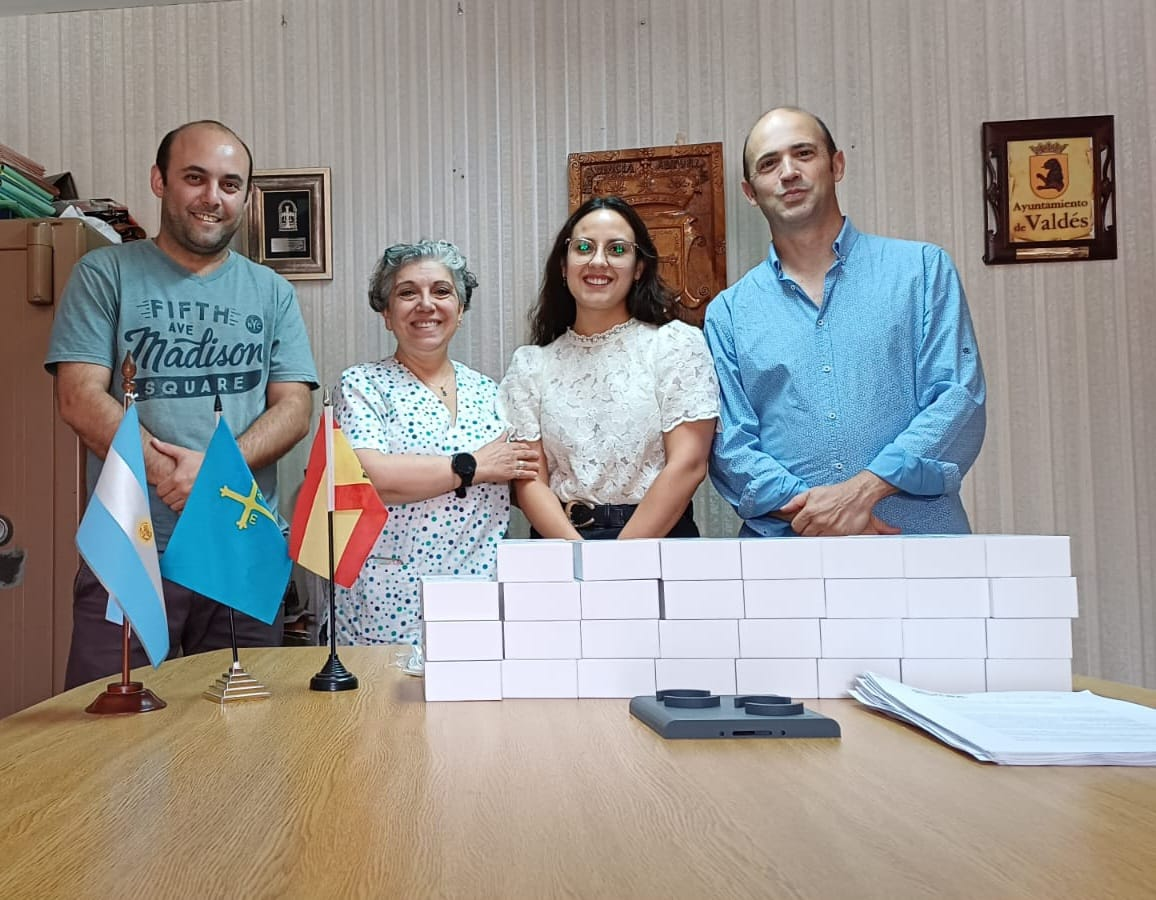
\includegraphics[width=0.8\textwidth]{./fotos/entrega_relojes.jpeg}
\caption{Entrega de los relojes ID Vita en la Residencia Asturiana, durante el primer día de la implementación, junto al equipo del proyecto y la médica responsable.}
\end{figure}

\subsection{El conjunto de datos}
La información la provee la empresa proveedora de los relojes (Intelligent Data), que remite los datos de los residentes una vez por semana. Llegan como un volcado (\textit{dump}) de una base de datos MySQL/MariaDB, generado con \texttt{mysqldump} y de un tamaño cercano a los 500 MB. Sobre ese volcado se trabajó de forma reproducible (el procesamiento se detalla en el Capítulo 6).\\

El volcado contiene varias tablas, aunque solo dos concentran la información efectivamente utilizada. La Tabla 1 resume su contenido.\\


\begin{table}[h!]
\centering
\begin{tabular}{lrl}
\hline
Tabla & Filas & Observación \\
\hline
\texttt{patients} & 26 & 22 con datos de wearable asociados \\
\texttt{wearabledata} & 2.363.501 & serie temporal de signos vitales \\
\texttt{perceivedhealthdata} & 122 & estado auto-percibido (no usado aún) \\
\texttt{clinicalevents} & 0 & vacía en el volcado \\
\texttt{labresults} & 0 & vacía en el volcado \\
\texttt{sessionresults} & 0 & vacía en el volcado \\
\hline
\end{tabular}
\caption{Tablas presentes en el volcado de datos recibido.}
\end{table}
El grueso del trabajo recae sobre \texttt{wearabledata}: más de 2,36 millones de registros que conforman las series temporales de seis métricas. La Tabla 2 muestra su distribución. Las cinco variables fisiológicas tienen una cobertura muy pareja (cercana a los 468.000 registros cada una), mientras que los pasos diarios aparecen con una frecuencia mucho menor.\\


\begin{table}[h!]
\centering
\begin{tabular}{lr}
\hline
Métrica & Registros \\
\hline
Temperatura & 468.589 \\
Presión diastólica & 468.589 \\
Presión sistólica & 468.588 \\
Frecuencia cardíaca & 468.587 \\
Saturación de oxígeno & 468.587 \\
Pasos diarios & 20.561 \\
\hline
\end{tabular}
\caption{Distribución de registros de \texttt{wearabledata} por métrica.}
\end{table}
Los relojes se entregaron en la Residencia en diciembre de 2025, de modo que el período de monitorización relevante para este trabajo abarca desde esa fecha hasta mediados de 2026: unos seis meses de datos densos por paciente, con el muestreo de cinco minutos ya mencionado. El volcado contiene además registros anteriores —que se remontan hasta 2023—, ajenos a la monitorización del proyecto y sin relevancia para este trabajo. De cada registro se conserva únicamente lo necesario para la visualización y el análisis: el identificador del dispositivo, la métrica, la marca temporal y el valor.\\


\subsubsection{Limitaciones de los datos}
Trabajar con datos reales implica reconocer sus imperfecciones, y varias de ellas condicionaron decisiones de diseño que conviene explicitar:\\


\begin{itemize}
\item~ \textbf{Comorbilidades aún no cargadas.} Los campos de índice de Charlson, índice de Barthel y fecha de diálisis no se encuentran completados en los registros, y el de diabetes figura en cero para todos los pacientes; su carga corresponde al equipo clínico y queda pendiente. Por ese motivo no fue posible, por el momento, estratificar el análisis por comorbilidad, aunque su incorporación a futuro lo habilitaría.
\item~ \textbf{Presión arterial sospechosa.} Los valores de presión llegan desde el propio volcado ya confinados a un rango fijo y estrecho —la sistólica entre 90 y 139 mmHg, la diastólica entre 60 y 89 mmHg—, sin las excursiones que sí muestran las demás variables: la frecuencia cardíaca, por ejemplo, abarca de 42 a 151 bpm sobre los mismos datos. Esta acotación no la introduce la aplicación, sino que viene en el dump de la base, lo que sugiere que se trata de datos sintéticos. Por esa razón, la presión se visualiza pero se excluye del módulo de análisis de patrones.
\item~ \textbf{Pasos sin garantía de exactitud.} El fabricante no garantiza la precisión del conteo de pasos, por lo que también se excluyen del análisis, aunque pueden visualizarse.
\end{itemize}
Estas limitaciones se retoman en las conclusiones (Capítulo 9), donde pesan sobre la interpretación clínica de los resultados.\\


\subsection{Herramientas de desarrollo}
La herramienta se construyó íntegramente en Python, apoyándose en un conjunto acotado de librerías de código abierto. La Tabla 3 lista las principales, con las versiones efectivamente utilizadas y validadas.\\


\begin{table}[h!]
\centering
\begin{tabular}{lll}
\hline
Tecnología & Versión & Propósito \\
\hline
Python & 3.11+ & Lenguaje principal \\
Dash & 3.3.0 & Framework web reactivo \\
dash-bootstrap-components & 2.0.4 & Componentes de interfaz (tema oscuro) \\
pandas & 2.3.3 & Manipulación de series temporales \\
Plotly & 6.5.2 & Gráficos interactivos \\
pyarrow & 18.1.0 & Lectura/escritura de Parquet \\
gunicorn & 23.0.0 & Servidor de producción \\
fpdf2 & 2.8.7 & Generación de informes PDF \\
matplotlib & 3.10.8 & Gráficos de los informes \\
Flask / Werkzeug & (deps. de Dash) & Servidor base y hashing de contraseñas \\
\hline
\end{tabular}
\caption{Stack tecnológico principal.}
\end{table}
La elección de Dash junto con Plotly respondió a que están pensados para aplicaciones analíticas: integran gráficos científicos interactivos sin necesidad de programar en JavaScript y organizan la lógica de la interfaz en \textit{callbacks} reactivos. El resto de las decisiones tecnológicas (en particular el uso de Parquet y de un servidor liviano) estuvieron motivadas por una restricción concreta de hardware que se explica en el Capítulo 6.\\


\subsection{Relevamiento de requerimientos}
El diseño de la interfaz no partió de supuestos propios, sino de un relevamiento estructurado de las necesidades del equipo de salud. Antes de comenzar el desarrollo se elaboró un cuestionario de diseño, respondido por la médica responsable de la Residencia, orientado a entender el objetivo clínico, las métricas prioritarias, la organización de la pantalla principal, el flujo de uso y las escalas temporales. Las decisiones de diseño que se describen en el Capítulo 6 se apoyan directamente en sus respuestas.\\

En cuanto al objetivo, la herramienta se concibió como una medida preventiva: prestar atención a las variaciones de los signos vitales y programar el seguimiento del paciente ante la eventual aparición de una patología. Dentro de ese marco, la médica identificó la frecuencia cardíaca como la información más útil para el seguimiento, por su relación con la fiebre, la deshidratación y las variaciones de presión, y su vínculo con la saturación de oxígeno.\\

Un aspecto particularmente relevante surgió al consultar qué variable mostrar en primer lugar. La médica descartó tanto la temperatura como la saturación de oxígeno para ese rol, con un argumento clínico preciso: en los adultos mayores, la piel más fina y la baja temperatura periférica degradan la fiabilidad de esas mediciones. Señaló que la temperatura podía aprovecharse de todos modos mediante umbrales de fiebre o hipotermia, pero que la frecuencia cardíaca reflejaba mejor las variaciones fisiológicas. Esta observación, hecha por la propia usuaria clínica antes de iniciar el desarrollo, coincide con las limitaciones de la fotopletismografía en la población geriátrica discutidas en el marco teórico (Capítulo 3), y reaparecería más tarde en la evaluación de usabilidad (Capítulo 8).\\

Respecto de qué interesa observar de cada variable, la prioridad fue la comparación contra el valor basal del propio paciente, antes que contra un rango poblacional general. Esta definición —mirar a cada paciente respecto de su propio patrón— es la que dio origen al módulo de línea base personalizada.\\

Para la pantalla principal, la preferencia fue un resumen global del estado de la cohorte —cuántos pacientes están en alerta—, con la última semana como ventana de referencia. En cuanto al flujo de uso, la médica indicó que, al ingresar, lo que busca la mayoría de las veces es ver quién está en alerta, y que prefiere seleccionar primero un paciente y luego ver todas sus variables. También anticipó que habría otros usuarios además de ella, como personal de la administración de la Residencia.\\

Sobre las escalas de tiempo, se definió un rango por defecto de los últimos siete días, con un mes disponible a un clic. Para el seguimiento clínico, la médica priorizó los promedios por hora, día o rango horario por sobre los valores crudos, y eligió la línea temporal como el formato visual más útil.\\

Este relevamiento inicial permitió, además, identificar las tareas de revisión típicas del equipo de salud, que luego se usaron tanto para guiar el desarrollo como para la evaluación de usabilidad: la revisión semanal, la nocturna y la posterior a un evento clínico. A lo largo del desarrollo iterativo, algunas decisiones se refinaron a partir de la retroalimentación clínica; un ejemplo es el ajuste del umbral mínimo de temperatura, rebajado para evitar que las lecturas bajas habituales del sensor periférico se marcaran como alarma. El cuestionario de diseño completo se incluye en los anexos.\\


\subsection{Metodología de desarrollo}
El desarrollo siguió un enfoque iterativo y centrado en el usuario, con ciclos sucesivos de diseño, prueba y ajuste. Cada avance se contrastó con la mirada del equipo médico, incorporando su retroalimentación antes de seguir construyendo. Este ida y vuelta explica por qué la herramienta creció bastante más allá de su versión inicial: lo que empezó como un visualizador de series temporales con filtros fue sumando, a pedido y por necesidad, un sistema de alarmas, un módulo de análisis y la posibilidad de exportar informes. Todas las iteraciones del desarrollo se versionaron en un repositorio privado de GitHub, lo que permitió conservar el historial completo de los cambios y recuperar versiones anteriores cuando fue necesario.\\

La validación final de la usabilidad con el equipo de salud —mediante tareas representativas, registro de tiempos y errores, y una encuesta estandarizada— constituye una etapa metodológica propia y se detalla en el Capítulo 7.\\


\subsection{Consideraciones éticas}
El trabajo con datos de salud de una población vulnerable exigió un manejo cuidadoso de la información. Los datos de los residentes utilizados para alimentar la plataforma están anonimizados, evitando que los estudiantes o terceros puedan identificar a personas concretas. Se respetaron los protocolos de la institución y del proyecto de investigación en cuanto al resguardo de la confidencialidad, el almacenamiento seguro y el acceso restringido, aplicando un criterio de minimización: se limitó la recolección, el almacenamiento y la circulación de información a lo estrictamente necesario para el objetivo del proyecto. Por último, la participación del personal de salud en las entrevistas y en las pruebas de usabilidad fue voluntaria, con información clara sobre los objetivos del estudio y sobre el uso que se haría de los resultados.\\


\section{Implementación de la interfaz}
Este capítulo describe cómo se construyó VITAICARE: desde la arquitectura general y el pipeline que hace viable trabajar con millones de registros, hasta las vistas que usa el equipo médico, el sistema de alarmas, el módulo de análisis y, finalmente, el despliegue del sistema en producción. A lo largo del capítulo se señalan las decisiones de ingeniería que estuvieron motivadas por restricciones reales, porque son esas decisiones —y no la mera enumeración de funcionalidades— las que dan forma al resultado.\\


\subsection{Arquitectura general}
El sistema se organiza en tres capas. La \textbf{capa de presentación}, construida con Dash y \textit{dash-bootstrap-components} sobre un tema oscuro, contiene las dos vistas principales —el \textit{dashboard} de cohorte y el monitor por paciente— y un \textit{login} que intercepta toda petición sin sesión válida. La \textbf{capa de lógica o de dominio} concentra el procesamiento: la carga y el filtrado de datos, la detección de alarmas, el análisis de patrones, la generación de informes y la autenticación, con un cacheo en memoria de todas las operaciones costosas. Por debajo, la \textbf{capa de datos} provee las series ya procesadas en formato Parquet.\\

El flujo completo, de extremo a extremo, parte del reloj ID Vita —que mide cada cinco minutos— y termina en la pantalla del equipo médico. Entre ambos extremos, los datos llegan como un volcado SQL de la base MySQL de la empresa proveedora de los relojes, pasan luego a un formato intermedio (JSON) y finalmente a dos archivos Parquet livianos que la aplicación lee. Un detalle deliberado de esta arquitectura es que el procesamiento pesado se ejecuta en la PC de desarrollo, donde sobra memoria, mientras que el equipo que sirve la aplicación solo lee los archivos ya procesados.\\


\subsection{Pipeline de datos}
El pipeline es la pieza central de ingeniería del proyecto, y conviene entender el problema que resuelve antes que su mecánica. El volcado de la base pesa cerca de medio gigabyte. Cargarlo de forma directa en memoria agota la RAM del equipo de producción, una Raspberry Pi de apenas 2 GB. La solución fue transformar ese volcado en dos archivos columnar comprimidos, en tres etapas.\\

En la \textbf{primera etapa}, el volcado SQL se convierte a un formato intermedio. Como el archivo es demasiado grande para cargarlo entero, se implementó un analizador (\textit{parser}) que lo recorre línea por línea, sin tenerlo completo en memoria. Este analizador no se limita a partir el texto por comas: reconoce las comillas dentro de las cadenas, los caracteres de escape y los paréntesis anidados, de modo que no rompe las filas que contienen comas o paréntesis dentro de un valor de texto. Además, contabiliza las filas descartadas por desajuste de columnas, lo que permite auditar la integridad del volcado.\\

En la \textbf{segunda etapa}, ese formato intermedio se convierte a Parquet. Aquí ocurren tres operaciones clave: se conservan únicamente las cuatro columnas realmente utilizadas (identificador del dispositivo, métrica, marca temporal y valor), descartando el resto; se convierte la zona horaria de UTC a la hora de Argentina; y se normalizan los valores a tipo numérico. Es importante que esta preparación esté centralizada en una única función, compartida por el procesamiento por lotes y por el camino de respaldo, de modo que ambos produzcan exactamente el mismo resultado.\\

En la \textbf{tercera etapa}, la aplicación carga los Parquet. La función de carga prefiere siempre los archivos Parquet y solo recurre al formato intermedio si aquellos no existen (un escenario propio del desarrollo). Gracias a un cacheo, esa carga se paga una sola vez por proceso: la primera consulta asume el costo y las siguientes son instantáneas.\\

El impacto de esta decisión se resume en la Tabla 4. La reducción de unos 520 MB a unos 10 MB en disco, y de varios gigabytes a unos 280 MB en memoria, es exactamente lo que hace posible correr el sistema completo —con sus 2.363.501 filas— sobre hardware de bajo costo.\\


\begin{table}[h!]
\centering
\begin{tabular}{lll}
\hline
Métrica & Formato intermedio & Parquet \\
\hline
Tamaño en disco & $\sim$520 MB & $\sim$10 MB \\
RAM del DataFrame en memoria & varios GB (provoca OOM) & $\sim$280 MB \\
Tiempo de carga en la Pi & inviable & segundos \\
Columnas almacenadas & todas & solo 4 usadas \\
\hline
\end{tabular}
\caption{Efecto de la conversión a Parquet sobre el consumo de recursos.}
\end{table}

\subsection{Configuración centralizada}
Todo lo que el equipo médico podría querer ajustar vive en un único archivo de configuración, separado de la lógica. Esto incluye, ante todo, la definición de las seis métricas: su nombre, su color, su unidad y sus rangos normales. La Tabla 5 los recoge.\\


\begin{table}[h!]
\centering
\begin{tabular}{llrr}
\hline
Métrica & Unidad & Mínimo & Máximo \\
\hline
Frecuencia cardíaca & bpm & 50 & 120 \\
Saturación de oxígeno & \% & 80 & 100 \\
Presión sistólica & mmHg & 90 & 140 \\
Presión diastólica & mmHg & 60 & 90 \\
Temperatura & °C & 25,0 & 38,0 \\
Pasos diarios & pasos & 0 & (sin máximo) \\
\hline
\end{tabular}
\caption{Métricas monitorizadas y sus rangos normales por defecto.}
\end{table}
Sobre esta tabla cabe una aclaración metodológica que atraviesa todo el proyecto: \textbf{estos umbrales son valores por defecto razonables, no validados clínicamente}. Están centralizados y parametrizados precisamente para que el equipo médico los ajuste. El mínimo de temperatura, por ejemplo, se bajó de 33 °C a 25 °C a pedido de la médica, para evitar que las lecturas bajas habituales del sensor periférico se marcaran como alarma. La validación clínica de estos valores queda planteada como trabajo futuro.\\


\subsection{Autenticación y seguridad}
Dado que la herramienta maneja datos de salud, el acceso está protegido por un \textit{login} de usuario y contraseña. Un guardián de sesión intercepta toda petición: si no hay una sesión válida, redirige al formulario de ingreso. Las contraseñas no se guardan en texto plano, sino \textit{hasheadas}, en un archivo con permisos restringidos que no se versiona ni se sube al repositorio. La creación de usuarios se hace por línea de comandos directamente sobre el equipo de producción; como solo la administradora tiene acceso a ese equipo, solo ella puede dar de alta nuevos usuarios, y no existe un registro abierto en la web. La protección efectiva combina, entonces, el \textit{login} de la aplicación con el cifrado que aporta el proxy inverso de borde —que se describe más adelante, en el apartado de despliegue—, siempre sobre datos anonimizados.\\


\begin{figure}[h]
\centering
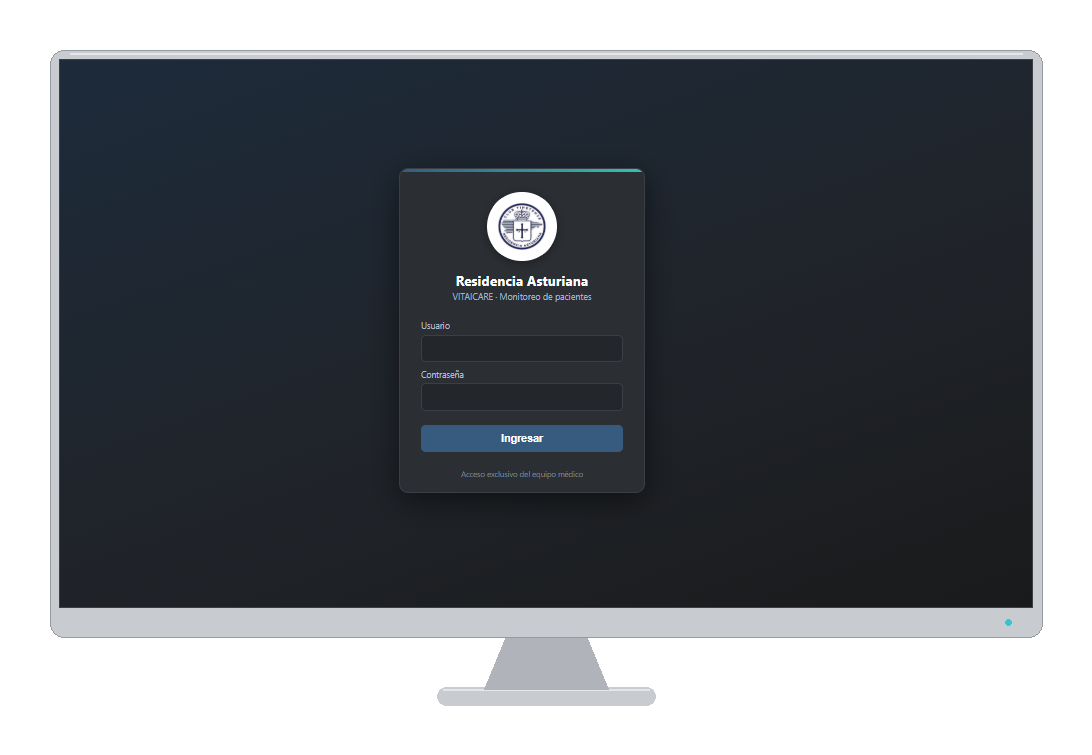
\includegraphics[width=\textwidth]{./png/login_monitor.png}
\caption{Pantalla de ingreso al sistema, protegida por usuario y contraseña.}
\end{figure}

\subsection{Las vistas de la interfaz}
La aplicación tiene dos vistas, pensadas para dos momentos distintos del trabajo clínico: una mirada panorámica de toda la cohorte y una mirada en profundidad de un paciente.\\


\subsubsection{Dashboard de cohorte}
Es la pantalla de entrada. Reúne un panel de alertas con tarjetas para los pacientes en estado crítico (hasta seis), una tabla resumen con todos los pacientes y su estado —últimos valores de frecuencia cardíaca, saturación, temperatura y presión sistólica—, y un acceso al historial de alarmas. Desde aquí, un clic sobre una tarjeta o una fila lleva directamente al monitor del paciente correspondiente. El historial se abre en una ventana modal, con filtro por métrica y la posibilidad de cargar semanas anteriores sin saturar la vista por defecto.\\


\begin{figure}[h]
\centering
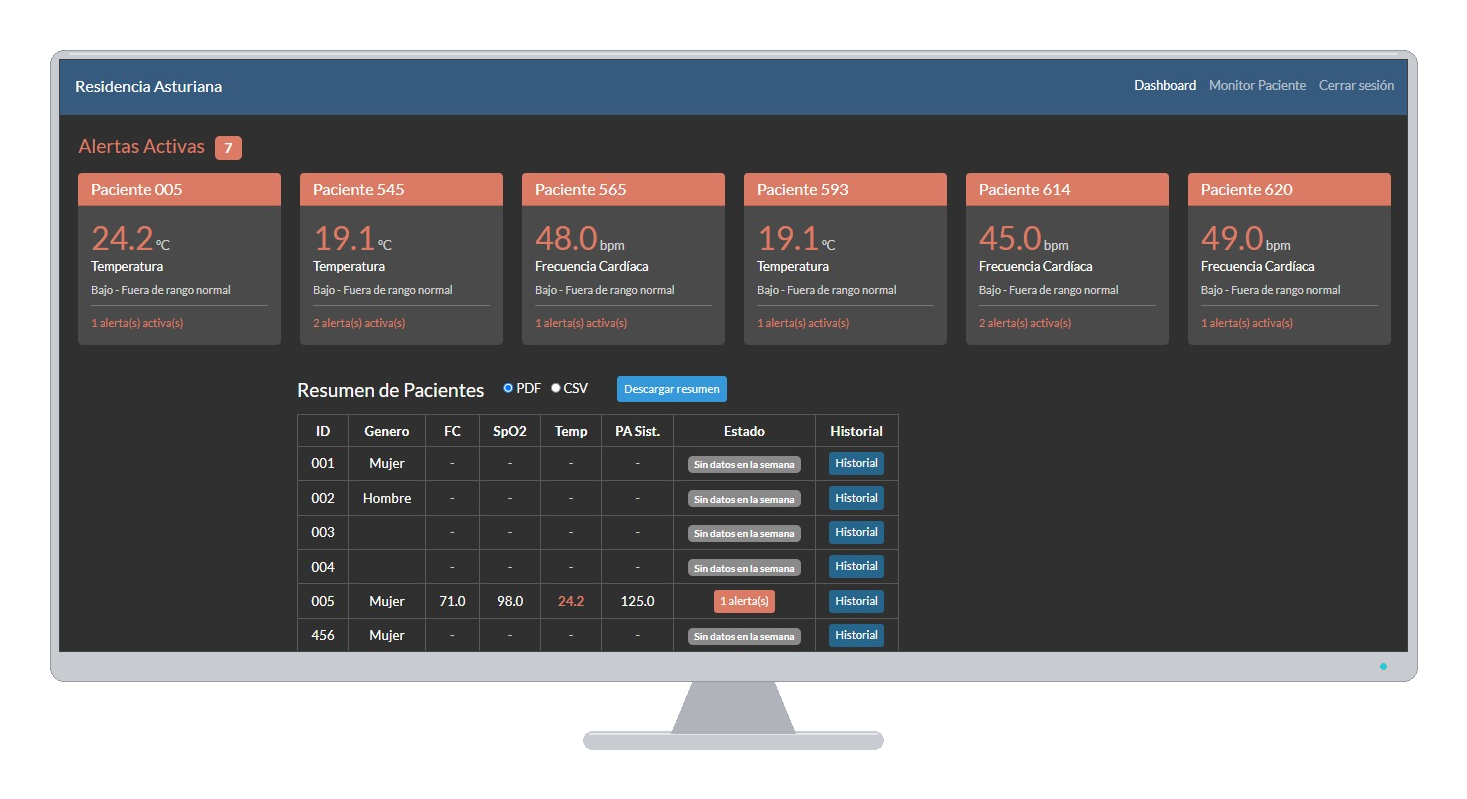
\includegraphics[width=\textwidth]{./png/principal.png}
\caption{Dashboard de cohorte: panel de alertas activas y tabla resumen del estado de todos los pacientes.}
\end{figure}

\subsubsection{Monitor de paciente}
Es la vista de detalle. Una barra lateral concentra los filtros —selección de paciente, fechas de inicio y fin, franja horaria, métricas a mostrar y modo de visualización— junto con la descarga de informes. El área principal presenta las estadísticas del período (mínimo, máximo y promedio por métrica) y el gráfico interactivo, que puede mostrar las métricas superpuestas en un mismo eje o separadas en subgráficos, según convenga a la comparación que se quiera hacer. Sobre el gráfico se despliega, además, una sección de análisis profundo con la línea base personalizada y las tendencias del paciente, que se describe más adelante.\\


\begin{figure}[h]
\centering
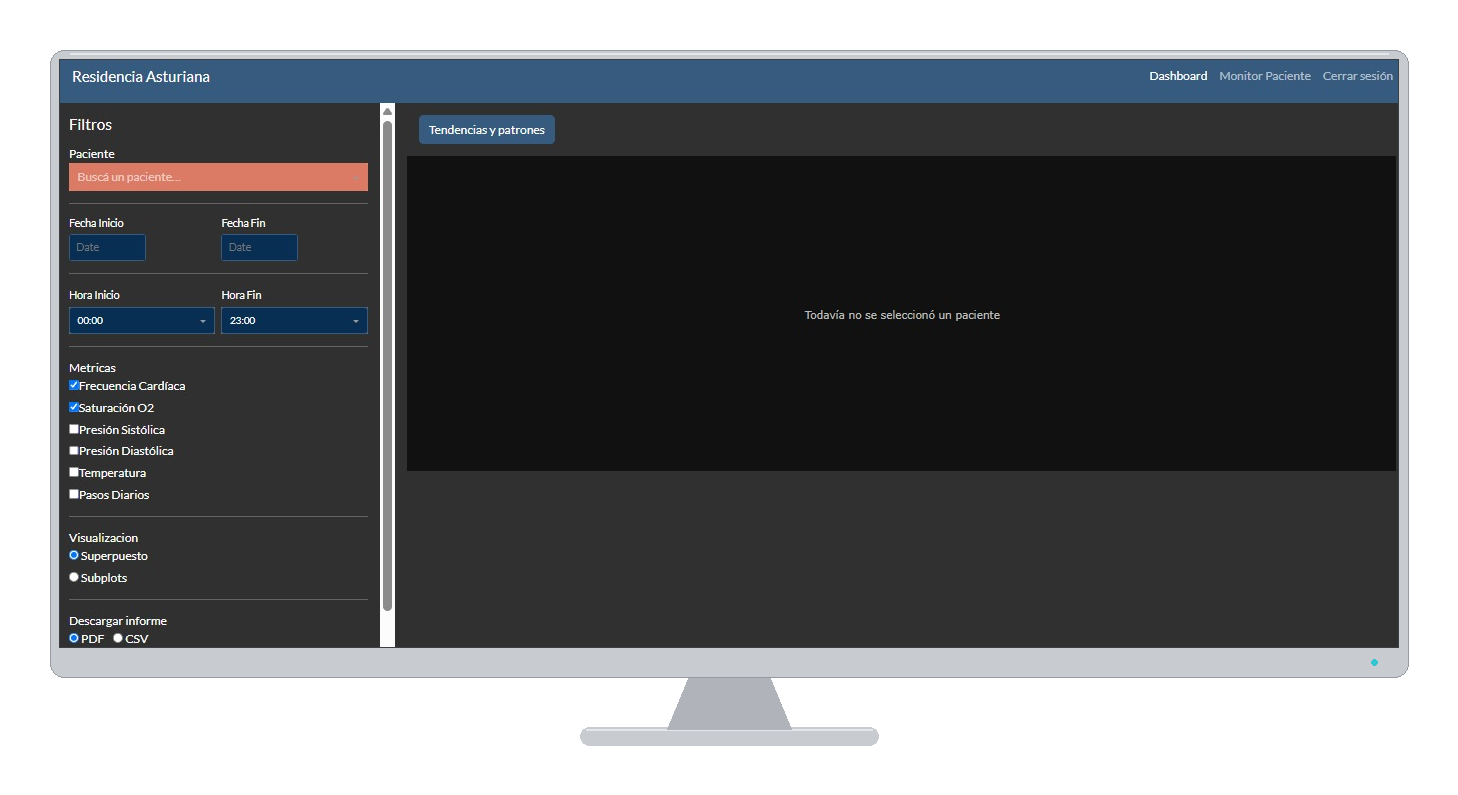
\includegraphics[width=\textwidth]{./png/genericobuscarpaciente.png}
\caption{Monitor de paciente: barra lateral de filtros, antes de seleccionar un residente.}
\end{figure}
Desde el dashboard de cohorte, al acceder a una alarma de un paciente —ya sea tocando su tarjeta de alerta o el botón “Ver” de su historial—, la aplicación navega directamente al monitor de ese paciente y lo posiciona sobre el evento. En lugar del período por defecto, muestra una ventana de dos horas antes y dos horas después de la alarma, marca con una cruz roja la lectura exacta que la disparó sobre el gráfico y deja seleccionadas varias métricas a la vez para poder correlacionarlas en ese momento. Este comportamiento responde directamente a un requerimiento del equipo médico.\\


\begin{figure}[h]
\centering
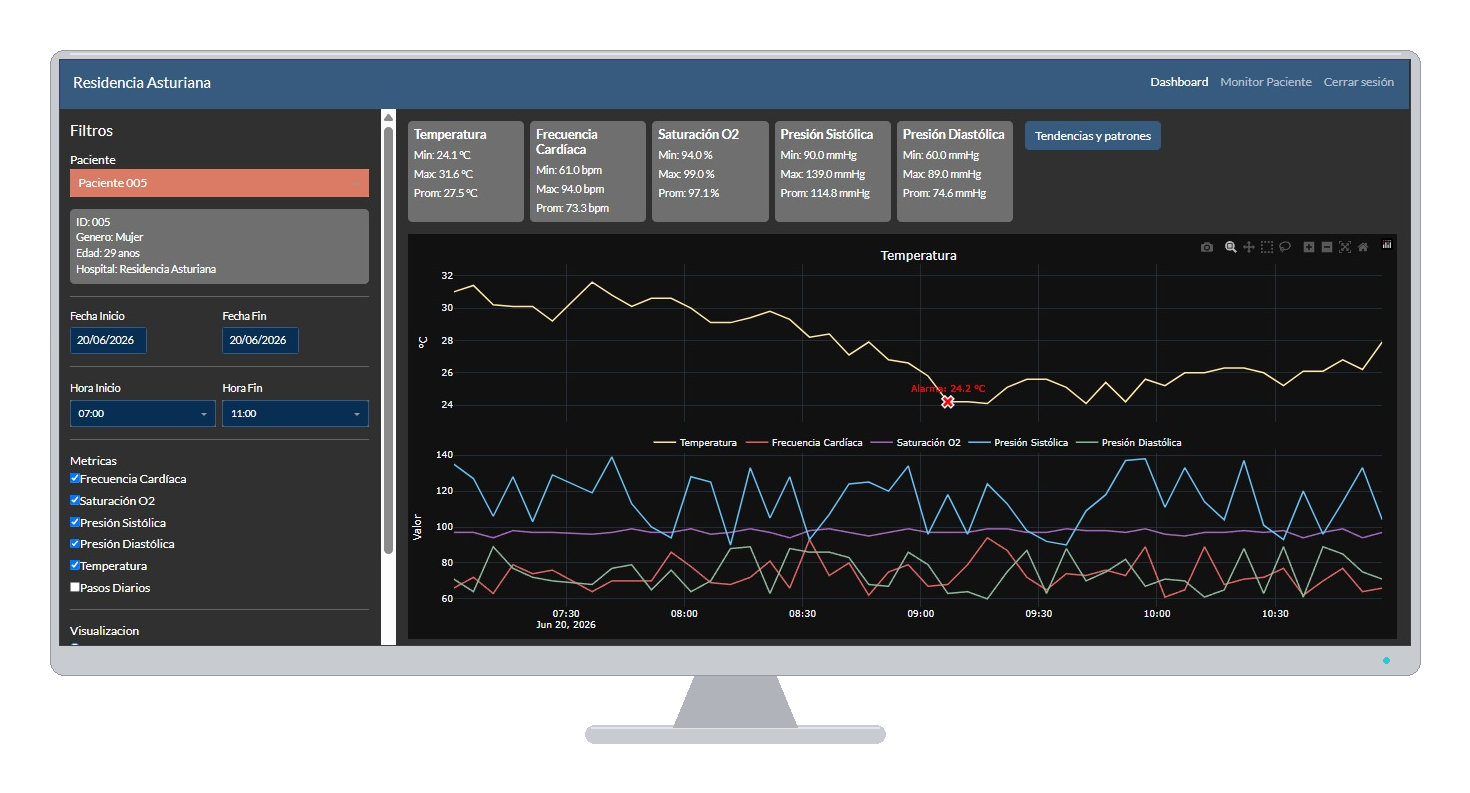
\includegraphics[width=\textwidth]{./png/alertapaciente005.png}
\caption{Monitor de un paciente alcanzado desde una alarma: ventana de dos horas antes y dos horas después del evento, con la lectura que disparó la alarma marcada con una cruz roja.}
\end{figure}

\subsection{Sistema de alarmas}
Una alarma, en su forma más simple, es un cruce de umbral: un valor por debajo del mínimo o por encima del máximo de su métrica. El problema es que, con un muestreo de cinco minutos, una condición sostenida —una saturación baja durante varias horas, por ejemplo— generaría decenas de alarmas idénticas y sepultaría la información útil bajo el ruido. La solución se construyó en dos niveles.\\

El primero es un \textbf{enfriamiento} (\textit{cooldown}): tras registrar una alarma, se ignoran las siguientes lecturas fuera de rango hasta que pase al menos una hora desde la última alarma conservada. Este enfriamiento se aplica de forma independiente por métrica y por tipo (alto o bajo), de modo que una métrica que oscila por encima y por debajo de su rango no se silencia a sí misma.\\

El segundo nivel es una \textbf{agrupación de eventos}: las alarmas consecutivas de una misma métrica y tipo, separadas por no más de hora y media, se colapsan en un único evento con su hora de inicio, su hora de fin, la cantidad de alarmas que lo componen y su valor más extremo. Así, una condición que dispararía “una alarma por hora” se presenta como un solo renglón legible —“de tal hora a tal hora”— en lugar de una lista interminable. Cada evento recuerda el momento de su alarma más extrema, que es justamente al que navega el botón de “Ver” del historial.\\

A las alarmas por cruce de umbral se suma un tercer tipo, de naturaleza distinta: la alarma de \textbf{falta de datos}. La revisión se acota a la última semana: si dentro de ese período el último registro de un paciente queda más de veinticuatro horas por detrás del dato más reciente del sistema —o si el paciente no tiene ningún registro en esa semana—, se interpreta que su reloj dejó de transmitir, por batería agotada, falta de sincronización o el dispositivo fuera de uso. La semana de referencia se ancla al dato más fresco del sistema, y no a la fecha actual, porque los datos son históricos. A diferencia de las alarmas de valor, esta condición no genera una tarjeta de alerta sino que se marca directamente en la tabla resumen de la cohorte.\\


\subsection{Módulo de análisis}
Más allá de los umbrales genéricos, el equipo médico estaba interesado en detectar cuándo un paciente se aparta de \textit{su propio} patrón. El módulo de análisis responde a esa necesidad con dos enfoques complementarios, aplicados sobre la frecuencia cardíaca, la saturación y la temperatura —se excluyen la presión y los pasos por las limitaciones de datos ya señaladas— y siempre tras descartar artefactos de medición.\\

El primero es la \textbf{línea base personalizada}. En lugar de un único rango igual para todos, se calcula el rango usual propio de cada paciente. Y como ese rango no es el mismo a lo largo del día —la frecuencia cardíaca nocturna difiere de la diurna—, se construye una banda circadiana: el día se divide en franjas de dos horas y, para cada una, se calculan los percentiles 10 y 90 del histórico del paciente. Los valores que caen fuera de esa banda se resaltan como “fuera de su patrón”. Cuando una franja no reúne suficientes datos, se recurre a una banda global de respaldo.\\


\begin{figure}[h]
\centering
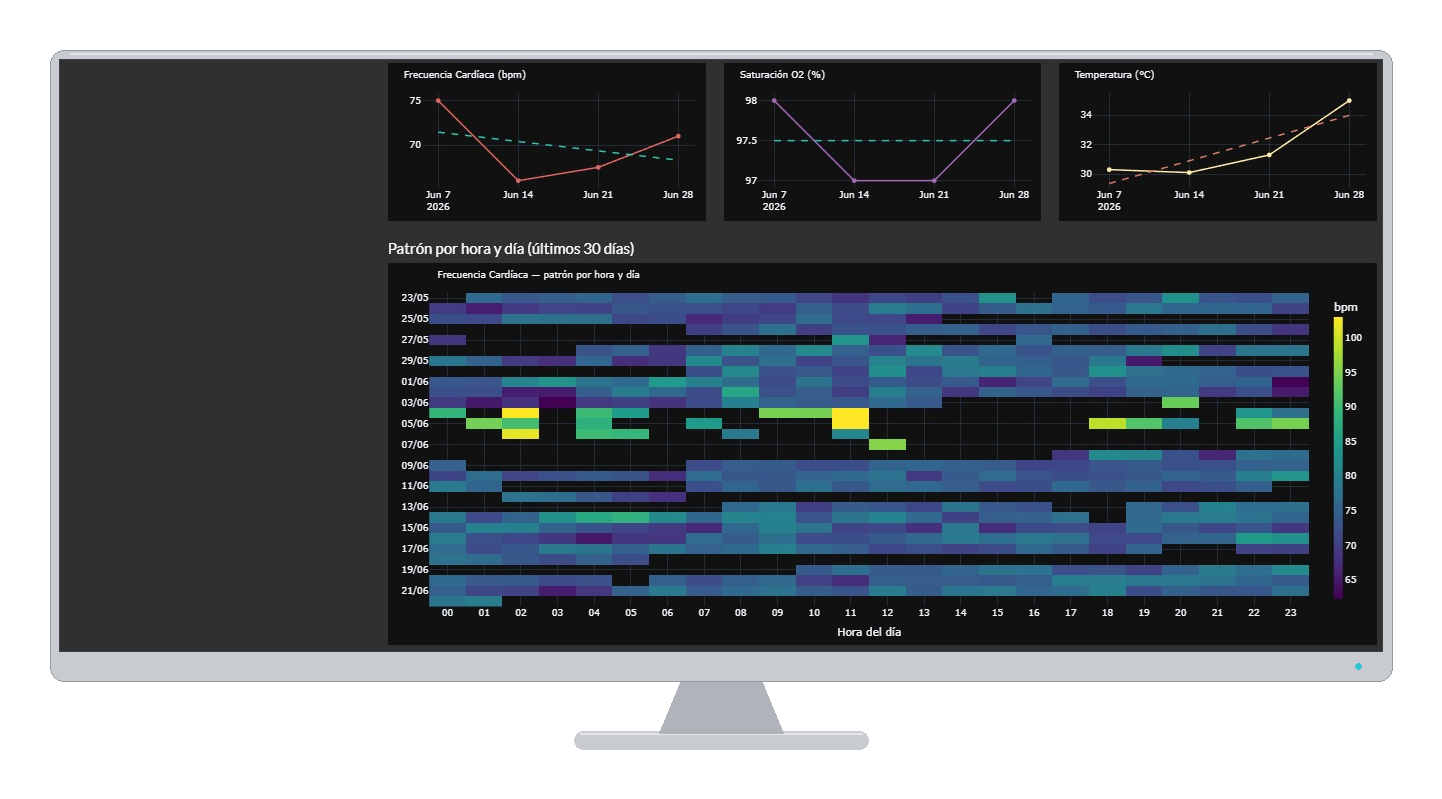
\includegraphics[width=\textwidth]{./png/patronpaciente005.png}
\caption{Línea base personalizada: patrón circadiano por hora y día del paciente (\textit{heatmap} de los últimos 30 días).}
\end{figure}
El segundo es la \textbf{detección de tendencias}, pensada como alerta temprana de deterioro sostenido. Para la frecuencia cardíaca se utiliza la frecuencia en reposo nocturna (el percentil bajo de las lecturas entre la medianoche y las seis de la mañana); para la saturación y la temperatura, la mediana diaria. Los valores se agregan por semana, se toman las últimas cuatro semanas y se ajusta una recta por mínimos cuadrados. Si la pendiente apunta en la dirección clínicamente adversa y supera un umbral mínimo, la tendencia se marca como adversa.\\


\begin{figure}[h]
\centering
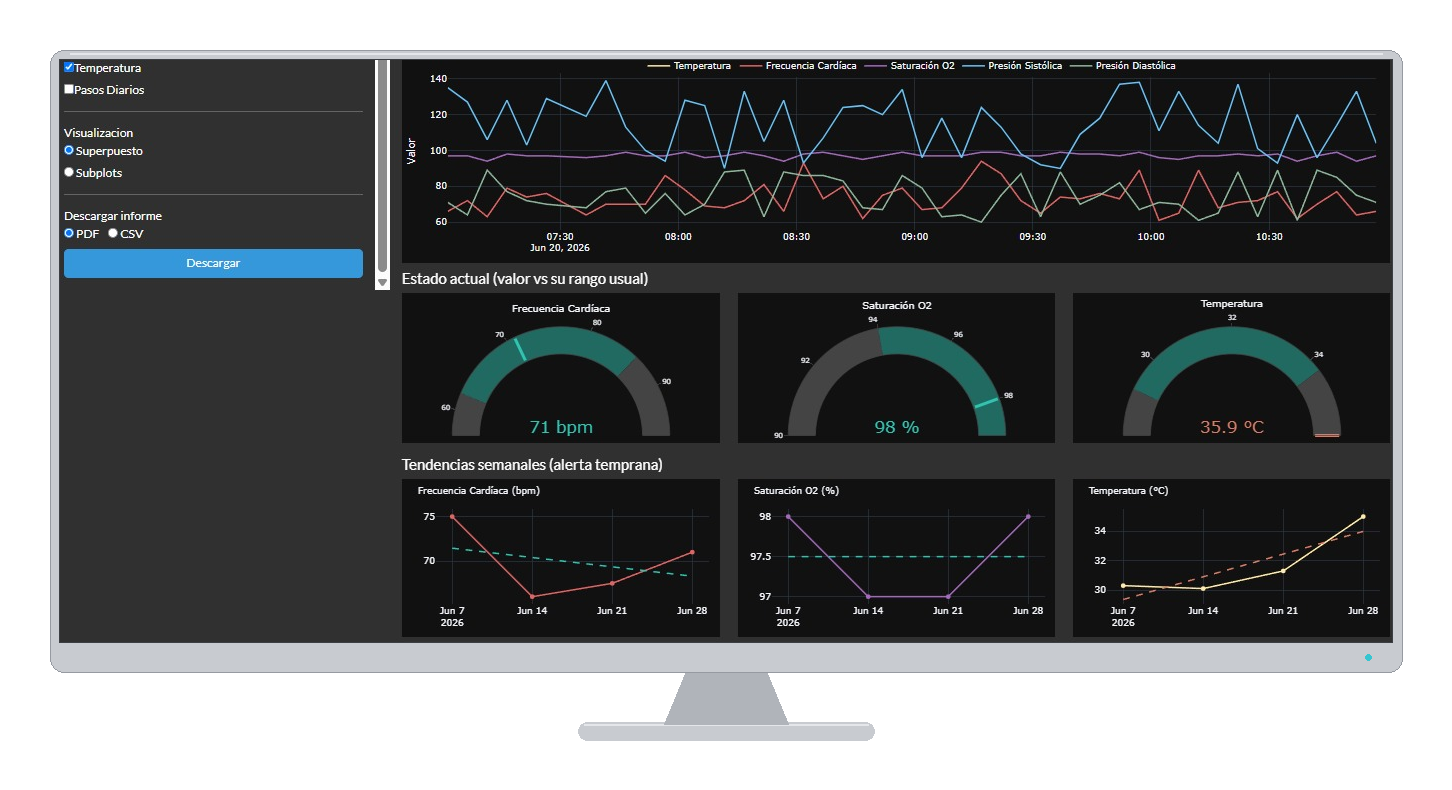
\includegraphics[width=\textwidth]{./png/tendenciaspaciente005.png}
\caption{Sección de análisis: estado actual sobre el rango usual del paciente (medidores) y tendencias semanales de alerta temprana.}
\end{figure}
Aquí aparece una decisión sutil pero importante: la ventana de análisis se ancla a la \textbf{última fecha de datos de cada paciente, y no a la fecha actual}. Como los datos son históricos y no llegan hasta hoy, anclar el análisis al presente descartaría información perfectamente válida.\\

Este módulo también obligó a una optimización de rendimiento. Una versión inicial, que filtraba el conjunto de 2,3 millones de filas una vez por cada combinación de paciente y métrica, tardaba unos 17,7 segundos. Reescribirla para hacer una única agrupación por métrica redujo ese tiempo a aproximadamente 1,8 segundos, casi diez veces más rápido, almacenando solo los parámetros resumidos en lugar de las series completas.\\


\subsection{Manejo de huecos en las series}
El reloj no siempre mide: hay períodos sin registros, ya sea porque el dispositivo estaba sin batería, en carga o fuera de la muñeca. Mostrar una línea continua a través de esos períodos sería engañoso, porque daría a entender que hubo mediciones donde no las hubo. Para evitarlo, antes de cada salto temporal mayor a un umbral se inserta un valor vacío que rompe la línea del gráfico. De este modo, la ausencia de datos se ve como una ausencia, y no como una continuidad ficticia de los signos vitales. La elección del umbral exacto para considerar que existe un hueco fue, en sí misma, una decisión de diseño discutida con el criterio clínico.\\


\subsection{Informes descargables}
El sistema permite exportar informes en PDF y en CSV, tanto por paciente como de toda la cohorte. El informe por paciente toma la selección activa del monitor e incluye los datos demográficos, una tabla de estadísticas, los eventos de alarma agrupados y, para cada evento (hasta un máximo de doce), un mini-gráfico de la métrica en una ventana que abarca desde dos horas antes hasta dos horas después del evento. El informe de cohorte resume a todos los pacientes con sus últimos valores y su estado, resaltando las filas en alerta. A modo de ejemplo, se adjuntan ambos informes —uno de cohorte y uno por paciente— en el Anexo, al final del documento.\\

La generación de estos informes tuvo que adaptarse a un entorno sin pantalla (\textit{headless}): se emplea un motor de gráficos que no requiere display y una librería de PDF escrita íntegramente en Python, evitando dependencias de sistema pesadas. Los archivos CSV se exportan con la marca de codificación adecuada para que los acentos se muestren correctamente al abrirlos en una planilla de cálculo.\\


\subsection{Despliegue en producción}
El sistema corre sobre una Raspberry Pi 4 de 2 GB con un sistema operativo de 64 bits. En producción, la aplicación se sirve con \texttt{gunicorn} (un \textit{worker} y dos \textit{threads}), un servidor WSGI gestionado por \textit{systemd}, lo que garantiza que arranque automáticamente al encender el equipo y se reinicie ante una falla; la ejecución directa con \texttt{python app.py} se reserva únicamente para el entorno de desarrollo. Se utiliza deliberadamente un único proceso de trabajo porque cada uno carga toda la serie de datos en memoria, y más de uno desbordaría los 2 GB disponibles. En este esquema, la aplicación sirve tráfico HTTP plano en un puerto interno y no se ocupa por sí misma del cifrado: esa responsabilidad se delega en la capa de borde de la red.\\

La Raspberry Pi que aloja la aplicación se encuentra dentro de una red local y no recibe el tráfico externo de forma directa. El acceso público se resuelve mediante un \textbf{proxy inverso}: las solicitudes dirigidas al dominio \texttt{vitaicare.whittileaks.com} llegan a un equipo de borde distinto —otra Raspberry Pi de la misma red, que actúa como puerta de entrada—, donde corre Caddy. Este proxy inverso administra la conexión segura por HTTPS y reenvía el tráfico hacia la Raspberry Pi de la aplicación, directamente al puerto HTTP en el que esta escucha. De este modo, el equipo médico accede desde un navegador común a través de una dirección pública y cifrada, mientras que el cifrado y la exposición a Internet quedan a cargo del proxy de borde, y la Raspberry Pi de la aplicación se concentra en servir el sistema.\\


\begin{figure}[h]
\centering
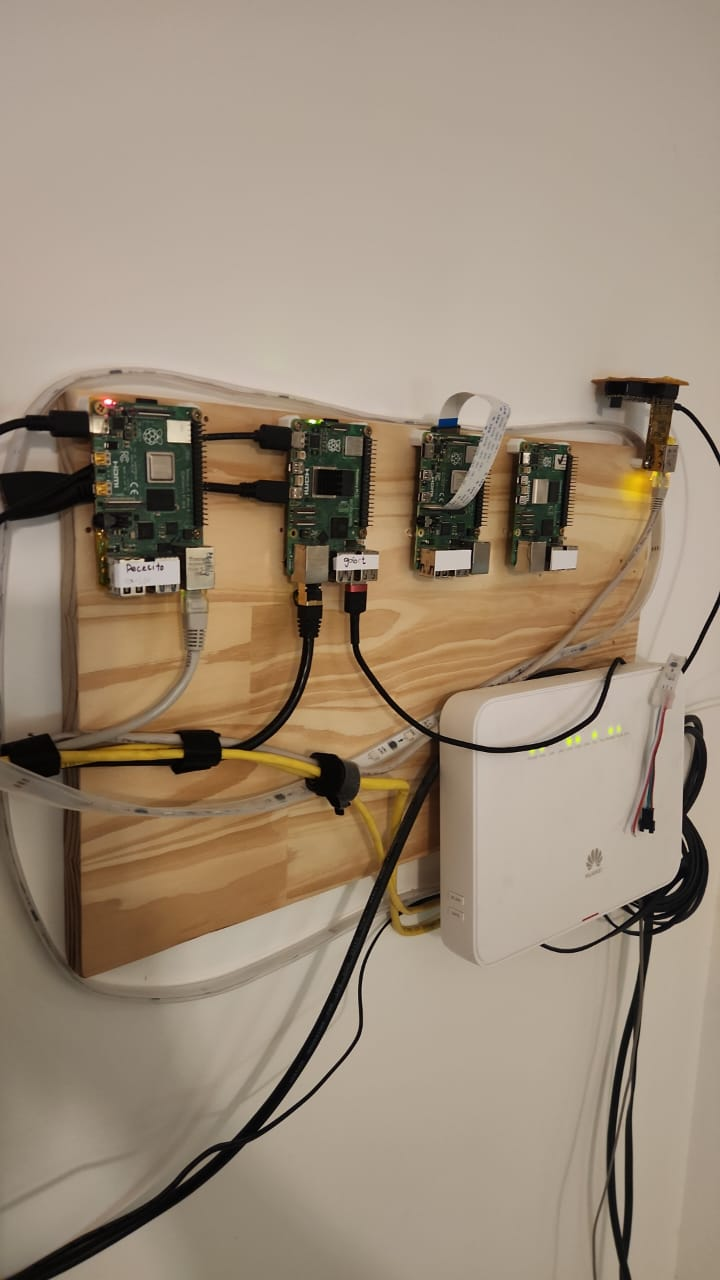
\includegraphics[width=0.5\textwidth]{./fotos/hardware.jpeg}
\caption{Infraestructura de despliegue: las Raspberry Pi —entre ellas la que sirve VITAICARE y la de borde con el proxy inverso— montadas junto al router de la red local.}
\end{figure}
El despliegue de nuevos datos se resuelve con un único comando que ejecuta todo el ciclo: convierte el volcado SQL, lo transforma a Parquet, sincroniza los archivos con el equipo de producción y reinicia el servicio para que tome los datos nuevos. Los pasos pesados de ese ciclo se ejecutan en la PC de desarrollo, y no en la Raspberry Pi, por la restricción de memoria mencionada.\\


\subsection{Síntesis de los desafíos técnicos}
Varios de los problemas resueltos a lo largo de la implementación comparten un rasgo: nacieron de restricciones reales y empujaron las decisiones de diseño más interesantes del proyecto. El más exigente —y el más cercano a la mirada de la Bioingeniería— fue el \textbf{manejo temporal y de la calidad de la señal}: el filtrado por franja horaria a través de la medianoche, resuelto combinando fecha y hora en un único instante con zona horaria; la distinción entre la ausencia de datos y una señal continua, para no dibujar mediciones donde no las hubo; y el descarte de artefactos y valores atípicos antes de cualquier análisis. Le siguió en peso la \textbf{memoria del hardware de bajo costo}, que motivó todo el pipeline a Parquet. Y junto a ellos, las \textbf{alarmas redundantes} en condiciones sostenidas, resueltas con enfriamiento y agrupación; el \textbf{análisis sobre datos históricos}, anclado a la última fecha de cada paciente; el \textbf{costo de analizar millones de filas}, reducido con una única agrupación y cacheo; la \textbf{generación de PDF sin pantalla}; y el \textbf{acceso seguro desde fuera de la institución}, sobre datos anonimizados. En conjunto, estas soluciones son las que convirtieron a VITAICARE de un visualizador a una plataforma de monitoreo desplegada y sostenible.\\


\section{Evaluación de usabilidad}
Construir una herramienta usable fue uno de los objetivos centrales de este trabajo, y la usabilidad no es algo que pueda darse por sentado: se pone a prueba observando a las personas usar el sistema para resolver tareas reales. Este capítulo describe cómo se diseñó esa evaluación; sus resultados se presentan en el Capítulo 8.\\


\subsection{Enfoque y alcance}
La evaluación siguió un enfoque de prueba de usabilidad moderada, combinando dos fuentes de información complementarias. Por un lado, la observación directa de los participantes resolviendo un conjunto de tareas representativas del uso real, con registro de su desempeño. Por otro, una medida estandarizada de la percepción global de usabilidad mediante la escala SUS (\textit{System Usability Scale}). A esto se sumaron preguntas abiertas para recoger impresiones cualitativas.\\

Conviene encuadrar el alcance con honestidad. En evaluación de usabilidad se considera que con cinco a ocho participantes se detecta la mayoría de los problemas de uso; este trabajo se realizó con cuatro participantes, por lo que sus resultados deben leerse en clave \textbf{exploratoria y cualitativa}, como una validación preliminar, y no como una medición con valor estadístico. Aun así, la elección de los participantes no fue casual: cubren los dos perfiles de usuario para los que se diseñó la herramienta —la mirada clínica y la del equipo de investigación—, a los que se suma la mirada del tutor del proyecto, desde el ámbito académico, lo que permite contrastar distintas miradas sobre el mismo sistema.\\


\subsection{Participantes}
Participaron cuatro personas, que cubren los dos perfiles de usuario del proyecto y suman una mirada académica:\\


\begin{itemize}
\item~ Una \textbf{médica de la Residencia Asturiana}, usuaria clínica final de la herramienta y responsable de las decisiones que el sistema busca apoyar.
\item~ Dos \textbf{investigadoras de la Universidad de Alcalá}, con un perfil más técnico, vinculadas al proyecto desde la línea de investigación en teleasistencia.
\item~ El \textbf{tutor del proyecto}, docente del Instituto Tecnológico de Buenos Aires, que aportó una mirada académica y de evaluación experta sobre la herramienta.
\end{itemize}
Esta combinación es deliberada: la mirada clínica aporta sobre la utilidad y la pertinencia de la información, la técnica sobre la navegación y el funcionamiento, y la académica sobre la claridad y la curva de aprendizaje. La participación de los cuatro fue voluntaria, con consentimiento informado y sobre datos anonimizados, conforme a las consideraciones éticas descritas en el Capítulo 5.\\


\subsection{Tareas}
Cada participante resolvió seis tareas, construidas a partir de las situaciones de uso típicas relevadas con el equipo de salud. Las tres centrales reproducen los escenarios clínicos identificados —la revisión semanal, la nocturna y la posterior a un evento—, y las restantes cubren la orientación general en el sistema, el análisis de tendencias y la exportación de informes:\\


\begin{enumerate}
\item~ \textbf{Orientación en el dashboard:} identificar, desde la pantalla principal, qué pacientes presentan alguna alerta en la semana.
\item~ \textbf{Revisión semanal:} consultar la evolución de la frecuencia cardíaca de un paciente en la última semana.
\item~ \textbf{Revisión post-evento:} mostrar la temperatura y la frecuencia cardíaca de un paciente durante la noche de un evento, en un mismo gráfico.
\item~ \textbf{Revisión nocturna:} analizar la franja nocturna de un paciente en los últimos días e identificar desviaciones respecto de lo habitual.
\item~ \textbf{Tendencias y patrón personal:} abrir la sección de análisis de un paciente y valorar si su patrón muestra algún deterioro.
\item~ \textbf{Exportar informe:} descargar el informe en PDF de un paciente.
\end{enumerate}

\subsection{Procedimiento e instrumentos de registro}
Tras leer el consentimiento, se enunció cada tarea en voz alta. El cronómetro se iniciaba cuando el participante comenzaba a actuar y se detenía cuando daba la tarea por resuelta; si requería ayuda, la tarea se anotaba como asistida. Durante la sesión se completó una \textbf{planilla de observación} que registró, por tarea, si se completó, el tiempo empleado, la cantidad de errores o desvíos —entendidos como clics equivocados, rutas incorrectas o dificultades para encontrar un control— y observaciones cualitativas, incluyendo frases textuales del participante.\\

Al finalizar, cada participante respondió el \textbf{cuestionario SUS} y cuatro preguntas abiertas (qué le resultó más útil, qué le resultó confuso, qué agregaría y si lo usaría en su trabajo diario). Las respuestas completas de los cuatro participantes se incluyen en el Anexo.\\


\begin{figure}[h]
\centering
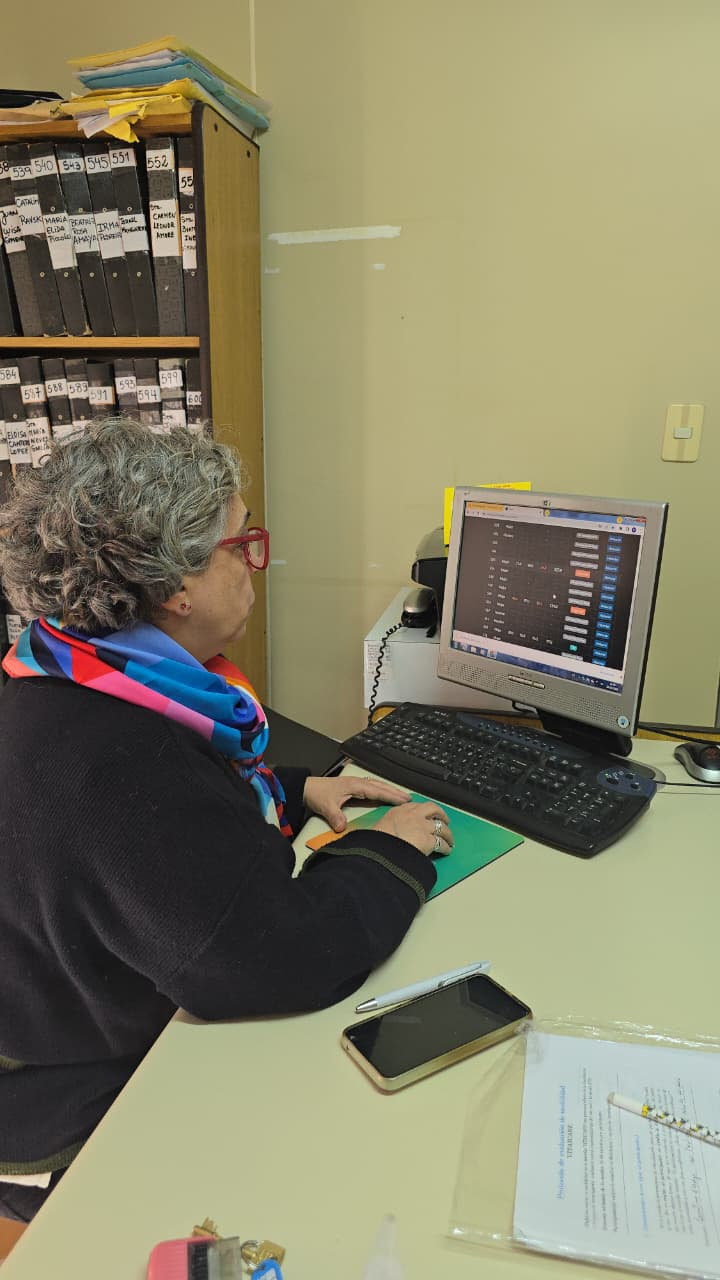
\includegraphics[width=0.45\textwidth]{./fotos/gladys_usando_app.jpeg}
\caption{La médica de la Residencia utilizando VITAICARE en su consultorio durante la evaluación de usabilidad.}
\end{figure}

\subsection{La escala SUS y su adaptación}
La SUS es un cuestionario estandarizado de diez afirmaciones que se responden en una escala de Likert de 1 (muy en desacuerdo) a 5 (muy de acuerdo), alternando afirmaciones positivas y negativas. Su resultado es un puntaje único de 0 a 100, comparable contra valores de referencia: el promedio histórico se ubica en torno a 68, y los valores por encima de 80 suelen considerarse excelentes.\\

En este trabajo se utilizó una versión adaptada al español, con una salvedad que conviene declarar: una de las diez afirmaciones se localizó al dominio clínico, reemplazando el ítem original por una afirmación positiva específica del contexto (“Consultaría el sistema para chequear valores clínicos luego de algún evento”). En consecuencia, el instrumento se reporta como una \textbf{adaptación de la SUS}. Para el cálculo del puntaje, cada afirmación se convierte en una contribución de 0 a 4 según su sentido —en las afirmaciones positivas, la contribución es el valor de la respuesta menos uno; en las negativas, cinco menos el valor—, y la suma de las diez contribuciones se multiplica por 2,5 para obtener el puntaje final. Este criterio respeta la lógica de la SUS y trata cada afirmación según su redacción efectiva.\\


\section{Resultados}
Este capítulo presenta los resultados del trabajo en dos planos: primero, lo que el sistema efectivamente logra como implementación; luego, lo que la evaluación de usabilidad reveló sobre su uso por parte del equipo de salud y de investigación.\\


\subsection{Resultados de la implementación}
El desarrollo alcanzó un sistema funcional, desplegado en producción y accesible de forma remota y segura. La Tabla 6 resume las funcionalidades implementadas.\\


\begin{table}[h!]
\centering
\begin{tabular}{ll}
\hline
Funcionalidad & Detalle \\
\hline
Pipeline de datos & Reproducible en un solo comando (SQL → JSON → Parquet) \\
Carga eficiente en la Pi & 2,36 M de filas con $\sim$280 MB de RAM \\
Dashboard de cohorte & Panel de alertas y tabla resumen \\
Monitor por paciente & Filtros, superposición/subgráficos y estadísticas \\
Sistema de alarmas & Umbral, enfriamiento de 1 h y agrupación de eventos \\
Historial navegable & Acceso directo al gráfico de cada evento \\
Línea base personalizada & Banda circadiana por percentiles, propia de cada paciente \\
Tendencias & Detección de deterioro sostenido por semana \\
Informes & Exportación en PDF y CSV, por paciente y de cohorte \\
Autenticación & Login y gestión de usuarios \\
Despliegue en producción & systemd y servidor WSGI en Raspberry Pi \\
Acceso remoto seguro & Proxy inverso con HTTPS y login de la aplicación \\
\hline
\end{tabular}
\caption{Funcionalidades implementadas en VITAICARE.}
\end{table}
En términos cuantitativos, el sistema procesa los 2.363.501 registros biométricos de los 22 pacientes con datos, sobre las seis métricas fisiológicas. La conversión del volcado a formato columnar reduce el almacenamiento de unos 520 MB a unos 10 MB y permite mantener el conjunto completo en memoria con cerca de 280 MB, lo que hace viable la ejecución sobre una Raspberry Pi de 2 GB. La optimización del módulo de análisis redujo el tiempo de cálculo de la vista general de aproximadamente 17,7 segundos, en una primera versión, a cerca de 1,8 segundos, casi diez veces más rápido.\\


\subsection{Resultados de la evaluación de usabilidad}
La evaluación se realizó con los cuatro participantes descritos en el Capítulo 7. Sus resultados se presentan en tres planos: el desempeño en las tareas, el puntaje de usabilidad percibida y los hallazgos cualitativos.\\


\subsubsection{Desempeño en las tareas}
Los cuatro participantes completaron la totalidad de las tareas sin asistencia. La Tabla 7 muestra el detalle por tarea. En conjunto, sobre veinticuatro tareas resueltas se registraron únicamente cuatro desvíos menores, y la mayoría de las tareas se completaron en segundos.\\


\begin{table}[h]
\centering
\footnotesize
\setlength{\tabcolsep}{4pt}
\begin{tabular}{c cc cc cc cc}
\hline
 & \multicolumn{2}{c}{\textbf{Médica}} & \multicolumn{2}{c}{\textbf{Investig. 1}} & \multicolumn{2}{c}{\textbf{Investig. 2}} & \multicolumn{2}{c}{\textbf{Tutor}} \\
\textbf{Tarea} & Tiempo & Err. & Tiempo & Err. & Tiempo & Err. & Tiempo & Err. \\
\hline
1 & 0:02 & 0 & 0:16 & 0 & 0:10 & 0 & 0:20 & 0 \\
2 & 0:46 & 0 & 2:00 & 1 & 0:12 & 1 & 0:30 & 1 \\
3 & 0:20 & 0 & 1:18 & 0 & 0:26 & 0 & 0:20 & 0 \\
4 & 0:22 & 0 & 0:30 & 0 & 0:50 & 0 & 0:45 & 0 \\
5 & 0:46 & 0 & 0:11 & 0 & 1:03 & 0 & 1:20 & 0 \\
6 & 0:25 & 1 & 0:15 & 0 & 0:11 & 0 & 0:15 & 0 \\
\hline
\end{tabular}
\caption{Desempeño por tarea (todas completadas sin asistencia). Tiempo en mm:ss.}
\end{table}
Los cuatro desvíos fueron leves y no impidieron completar la tarea. La médica, en la tarea de exportar el informe, buscó primero el control de descarga junto al gráfico antes de encontrarlo en la barra lateral. Los otros tres —las dos investigadoras y el tutor— tropezaron, en cambio, en la misma tarea de revisión semanal: realizaron un clic equivocado antes de retomar la ruta correcta, entrando primero al historial o a las alertas en lugar de seleccionar al paciente. Ninguno requirió ayuda.\\


\subsubsection{Usabilidad percibida (SUS)}
La Tabla 8 presenta las respuestas a la adaptación de la escala SUS y el puntaje resultante para cada participante.\\


\begin{table}[h]
\centering
\footnotesize
\setlength{\tabcolsep}{4pt}
\begin{tabular}{c l c c c c}
\hline
\textbf{Ítem} & \textbf{Afirmación (resumida)} & \textbf{Médica} & \textbf{Investig. 1} & \textbf{Investig. 2} & \textbf{Tutor} \\
\hline
1 & Usaría el sistema con frecuencia & 5 & 4 & 5 & 5 \\
2 & Lo encontré innecesariamente complejo & 1 & 1 & 1 & 2 \\
3 & El sistema es fácil de usar & 5 & 5 & 5 & 4 \\
4 & Necesitaría apoyo técnico & 1 & 1 & 1 & 4 \\
5 & Las funciones están bien integradas & 5 & 5 & 5 & 5 \\
6 & Lo consultaría tras un evento clínico & 5 & 5 & 5 & 5 \\
7 & La mayoría aprendería a usarlo rápido & 5 & 3 & 5 & 4 \\
8 & Lo encontré engorroso de usar & 1 & 2 & 1 & 2 \\
9 & Me sentí segura usándolo & 5 & 4 & 5 & 5 \\
10 & Necesité aprender mucho antes de empezar & 4 & 1 & 1 & 2 \\
\hline
\multicolumn{2}{r}{\textbf{Puntaje SUS}} & \textbf{92,5} & \textbf{87,5} & \textbf{100} & \textbf{80} \\
\hline
\end{tabular}
\caption{Respuestas a la adaptación de la SUS y puntaje por participante.}
\end{table}
Los puntajes obtenidos fueron de 92,5, 87,5, 100 y 80, con un \textbf{promedio de 90,0}. Los cuatro valores se ubican muy por encima del promedio histórico de referencia de la escala (cercano a 68) y dentro del rango considerado entre bueno y excelente. Más allá del número, las respuestas muestran un patrón coherente: el sistema se percibió como fácil de usar y bien integrado. Los puntos de menor acuerdo aparecen en torno a la curva de aprendizaje inicial y a la necesidad de apoyo, donde la médica y el tutor se diferenciaron de las dos investigadoras —un aspecto que se retoma a continuación.\\


\subsubsection{Hallazgos cualitativos}
Las observaciones y las respuestas abiertas resultaron especialmente informativas, y revelaron un contraste interesante entre los distintos perfiles.\\

En cuanto a lo \textbf{más valorado}, los cuatro coincidieron en la capacidad de la herramienta para volver legibles los datos, aunque cada perfil lo expresó a su manera: las investigadoras destacaron poder ver gráficamente la información —una de ellas señaló que “poder graficar todo de forma tan rápida permite identificar problemas mucho más ágilmente”—; la médica subrayó que le permite chequear de forma parcial o total a los residentes y, en algunos casos, anticipar eventos patológicos; y el tutor valoró la cantidad de datos disponibles y la libertad de uso, al no estar encapsulados en un análisis cerrado. Todos manifestaron que la usarían en su trabajo.\\

Los \textbf{puntos de fricción} difirieron según el perfil, y ahí está el hallazgo más rico. La médica señaló como confusa la calibración de algunos parámetros —puntualmente la temperatura, la frecuencia cardíaca y los pasos—. Las dos investigadoras, en cambio, coincidieron —de forma independiente— en un mismo punto de navegación: la comprensión del sistema de alertas; una no sabía dónde aparecerían los eventos en caso de haberlos, y la otra no tenía claro cuándo una alerta estaba activa ni a qué ventana temporal correspondía (la última semana, las últimas dos). El tutor, por su parte, apuntó a la curva de aprendizaje de los gráficos de patrón, que “requieren un tiempo de estudio”. En síntesis: la usuaria clínica reparó en la confianza sobre los valores, las usuarias técnicas en la legibilidad de las alertas y la navegación, y el tutor en la comprensión de las visualizaciones más complejas.\\

Respecto de \textbf{qué cambiarían}, una de las investigadoras no agregaría nada (“lo veo muy bien”) y la otra propuso aclarar el sistema de alertas; el tutor propuso sumar un menú de ayuda que explicara, en cada gráfico, de dónde salen los datos y qué hace cada control; y la médica propuso incorporar avisos activos de alerta —por ejemplo, una notificación por correo o un indicador de notificaciones en tiempo real—, una sugerencia concreta que se recoge entre las líneas de trabajo futuro.\\

Notablemente, el punto de fricción señalado por la médica —la confianza sobre la calibración de ciertos parámetros— coincide con las limitaciones de los datos identificadas de forma independiente durante el desarrollo (Capítulo 5), en particular respecto de la presión arterial y los pasos. La interpretación de estos hallazgos, y de las diferencias entre los distintos perfiles de usuario, se retoma en las conclusiones (Capítulo 9).\\


\begin{figure}[h]
\centering
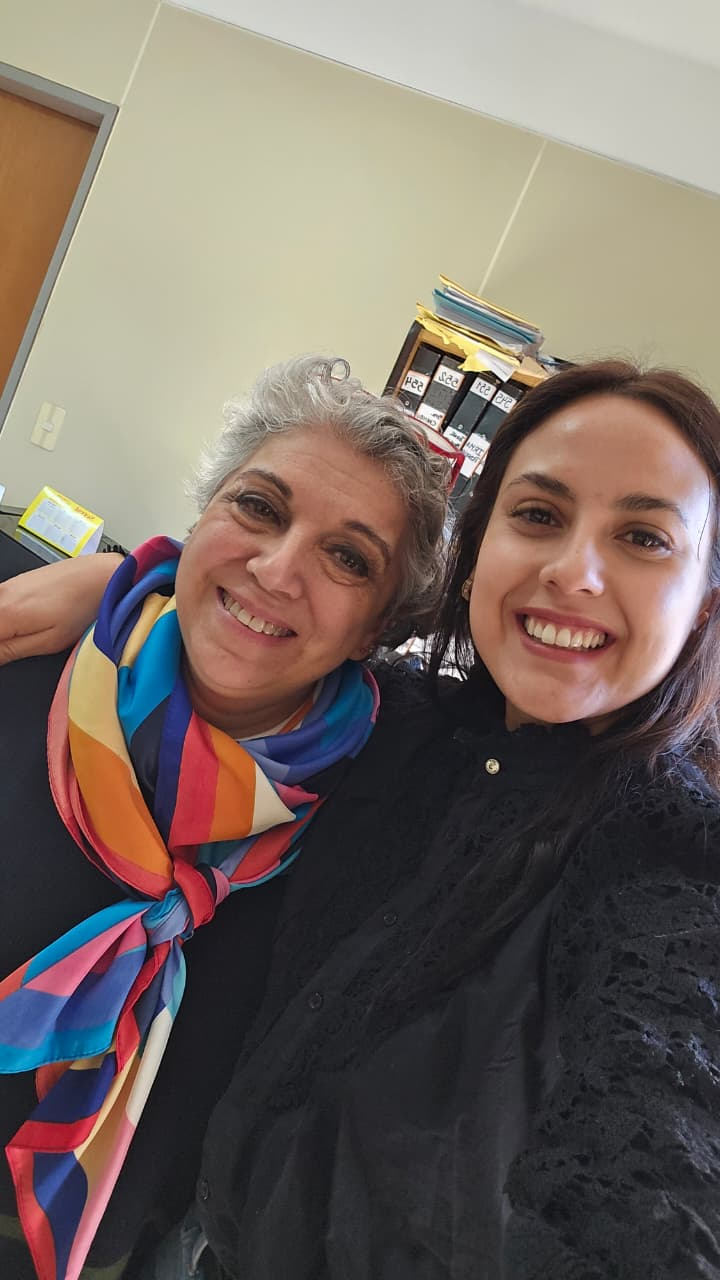
\includegraphics[width=0.45\textwidth]{./fotos/gladys_ultimodia.jpeg}
\caption{Cierre del trabajo de campo en la Residencia Asturiana, tras completar la evaluación de usabilidad final.}
\end{figure}

\section{Conclusión}
Este Proyecto Final de Carrera partió de una pregunta simple y a la vez difícil: cómo lograr que los datos biométricos de un grupo de personas mayores institucionalizadas dejaran de ser un volcado ilegible y llegaran al equipo de salud convertidos en información clara, comprensible y clínicamente útil. La respuesta tomó la forma de VITAICARE, una herramienta que empezó como un visualizador de series temporales con filtros y terminó siendo un sistema de monitoreo completo, desplegado en producción sobre hardware de bajo costo y accesible de forma remota y segura para el equipo de la Residencia Asturiana.\\

Los objetivos planteados al inicio se cumplieron. Se organizó la trazabilidad de los dispositivos, vinculando cada reloj con su paciente y su período de uso; se relevaron los requerimientos junto a la médica responsable, y de allí surgieron las decisiones de diseño centrales —desde priorizar la frecuencia cardíaca hasta mirar a cada paciente respecto de su propio patrón—; se definió una arquitectura en tres capas con un pipeline reproducible que vuelve viable trabajar con más de dos millones de registros en una Raspberry Pi de 2 GB; se construyó una interfaz funcional con sus dos vistas, su sistema de alarmas, su módulo de análisis y sus informes exportables; y se evaluó su usabilidad con los dos perfiles de usuario para los que fue pensada. Lo que se había propuesto como un prototipo verificable se convirtió, en el camino, en un sistema en uso real.\\

Ese resultado, sin embargo, debe leerse con la honestidad que exige el trabajo con datos clínicos. La fuente primaria es un dispositivo de consumo, y la fotopletismografía sobre la que se apoya pierde exactitud justamente en la población geriátrica —peor perfusión periférica, piel más fina, mayor prevalencia de arritmias—. Por eso, a lo largo de todo el proyecto, los datos del reloj se trataron como una señal de tendencia y de tamizaje, útil para orientar la atención del equipo de salud, y no como una medición de grado clínico. A esto se sumaron las limitaciones del propio conjunto de datos: la presión arterial llegaba desde el volcado acotada a un rango fijo —indicio de que se trataba de valores sintéticos—, el conteo de pasos no tiene precisión garantizada y varios campos de comorbilidad venían vacíos. De ahí que la presión y los pasos se visualicen pero se excluyan del análisis de patrones, y que los umbrales se hayan dejado como valores por defecto razonables, centralizados y parametrizados, a la espera de su validación clínica. Reconocer estos límites no debilita el trabajo: lo ubica con precisión en lo que es —una plataforma de visualización y soporte a la decisión— y en lo que todavía no es.\\

La evaluación de usabilidad, aunque exploratoria por su número de participantes, fue especialmente reveladora. Los puntajes obtenidos en la escala SUS —92,5, 87,5, 100 y 80, con un promedio de 90— ubican a la herramienta muy por encima del valor de referencia y dentro del rango considerado entre bueno y excelente. Pero el hallazgo más rico no estuvo en el número, sino en el contraste entre las distintas miradas: la usuaria clínica reparó en la confianza sobre la calibración de ciertos parámetros, las dos usuarias técnicas en la legibilidad de las alertas y la navegación, y el tutor en la curva de aprendizaje de las visualizaciones más complejas. Que la preocupación de la médica coincidiera, sin que ella lo supiera, con las limitaciones de los datos detectadas de forma independiente durante el desarrollo —la presión y los pasos— fue una de las confirmaciones más valiosas de todo el proceso: la intuición clínica y el análisis técnico señalaron, desde lugares distintos, exactamente el mismo punto.\\

Frente al estado del arte, donde la mayoría de las experiencias se detienen en la etapa de prototipo, el principal aporte de VITAICARE es haber llegado a desplegarse e integrarse en el flujo de trabajo de una residencia concreta, sobre hardware accesible y con una mirada centrada en el patrón propio de cada paciente. Quedan, naturalmente, líneas de continuidad claras: la validación clínica de los umbrales, la ingesta automática y en tiempo real de los datos —hoy procesados a partir de un volcado—, la correlación sistemática de las mediciones con eventos clínicos registrados, la incorporación de avisos activos de alerta —una notificación por correo o en tiempo real, tal como pidió la propia médica—, que, al tratarse ya de una aplicación web, podrían entregarse directamente en el navegador mediante la Web Notifications API, sin necesidad de desarrollar una aplicación dedicada; y la exploración de la escalabilidad hacia otros centros de cuidado, incluida la comparación con el centro de investigación de la Universidad de Alcalá.\\

Más allá de la arquitectura, del pipeline y de los puntajes, lo que este trabajo deja es algo más difícil de medir. Empezó llevando los relojes a la Residencia para entregarlos al equipo de salud, con sus cajas apiladas sobre una mesa, y terminó viendo a la médica usar el sistema en su propio consultorio para chequear a sus residentes, rodeada de las historias clínicas de siempre. En ese recorrido, una herramienta de software dejó de ser un ejercicio académico para volverse una pequeña parte del cuidado cotidiano de personas que necesitan que alguien las mire de cerca. El sentido de la Bioingeniería lo encontré en este trabajo, justamente ahí: en tender puentes entre el dato y la persona, entre la técnica y el cuidado. Que este proyecto final de carrera haya cruzado ese puente, aunque sea modestamente y en una sola residencia, es la conclusión que da por bien empleado todo el esfuerzo.\\



% =======================
% BIBLIOGRAFÍA (en nueva página)
% =======================
\clearpage
\printbibliography[title={Bibliografía}]

% =======================
% ANEXOS (en nueva página)
% =======================
\clearpage
\section*{Anexos}
\addcontentsline{toc}{section}{Anexos}

\subsection*{Anexo A. Informes de ejemplo generados por el sistema}

\noindent\textbf{Informe de cohorte (resumen de pacientes).} Es la descarga
disponible desde la vista general del \emph{dashboard}: reúne a todos los
pacientes con sus últimos valores y su estado, resaltando las filas en alerta.

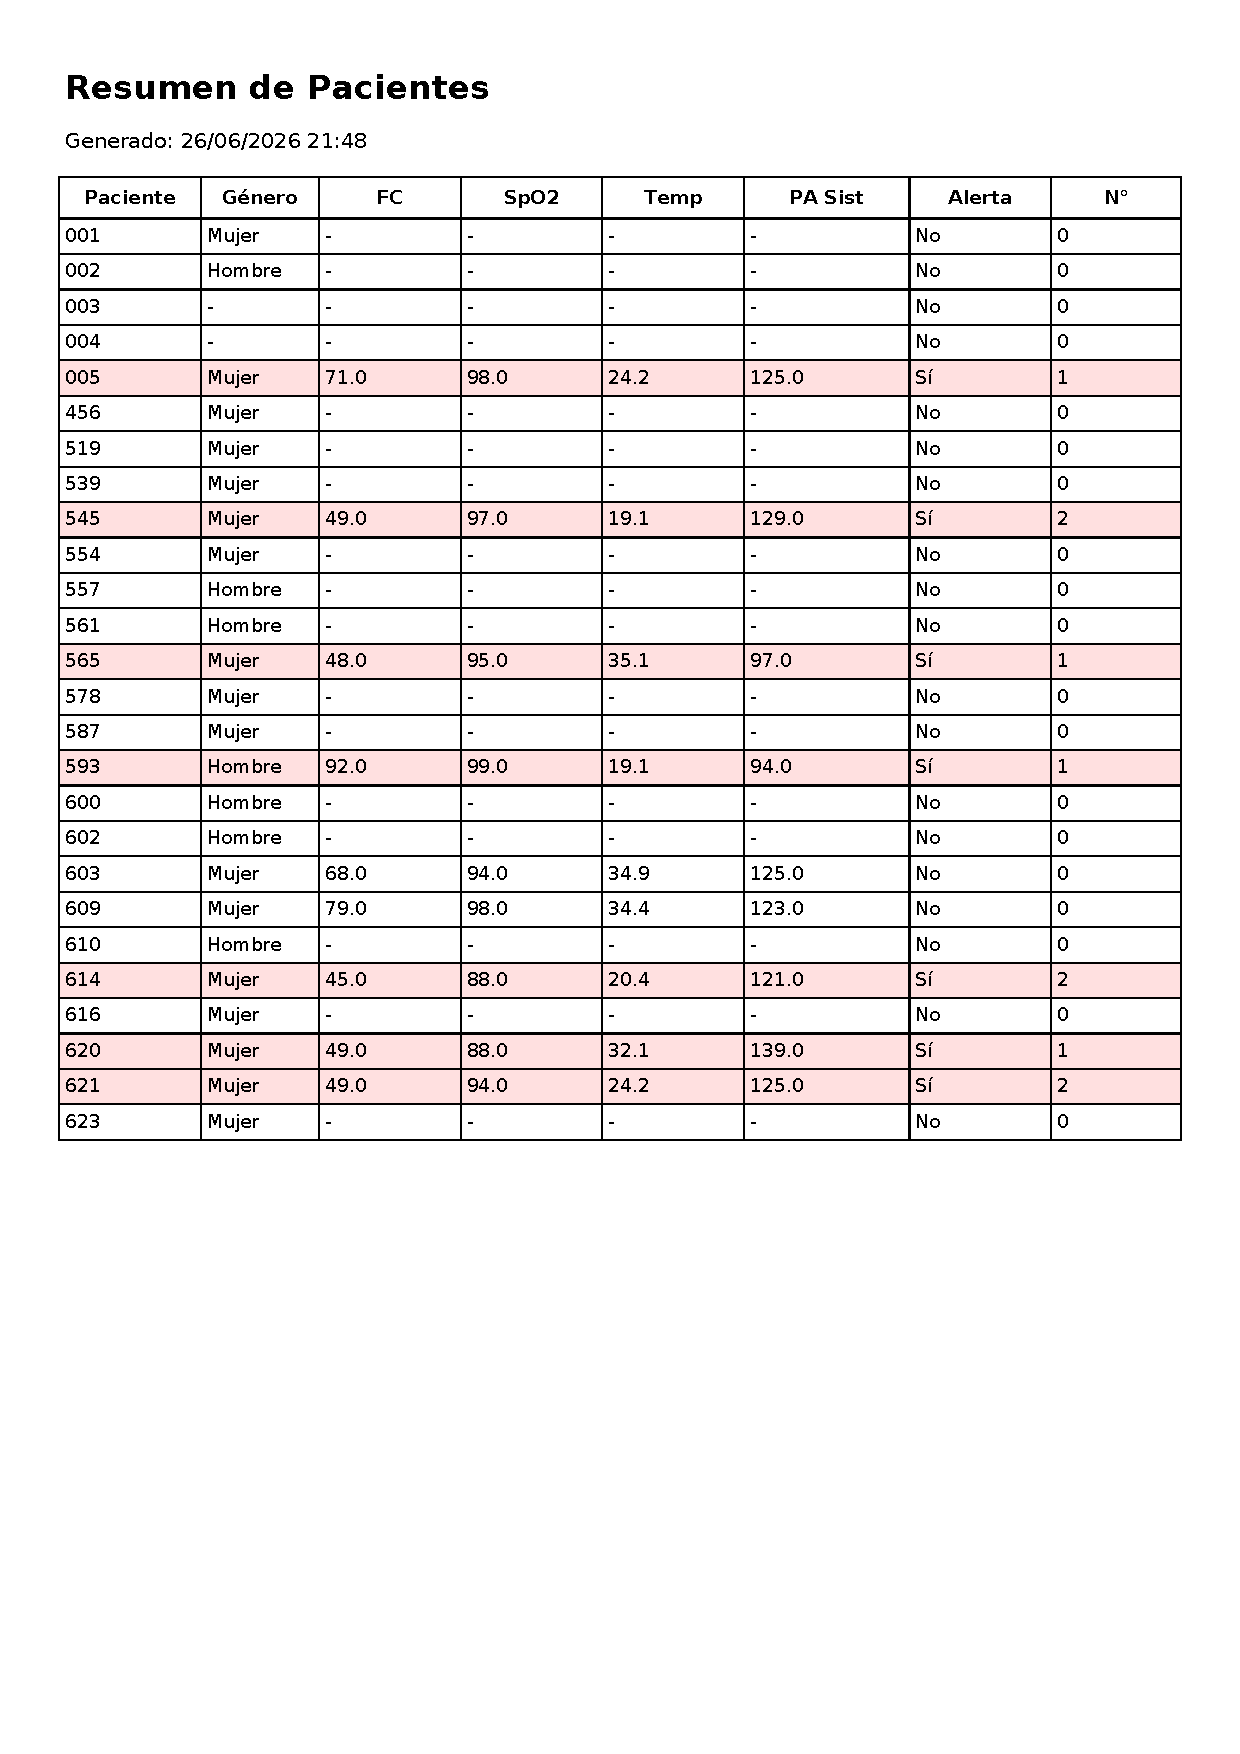
\includepdf[pages=-,pagecommand={\thispagestyle{plain}}]{./reportes/resumen_pacientes.pdf}

\noindent\textbf{Informe por paciente.} Es la descarga disponible desde el
monitor de un paciente —por ejemplo, al llegar a él para revisar una alarma—:
incluye sus datos, una tabla de estadísticas y los eventos de alarma agrupados,
con un gráfico alrededor de cada uno.

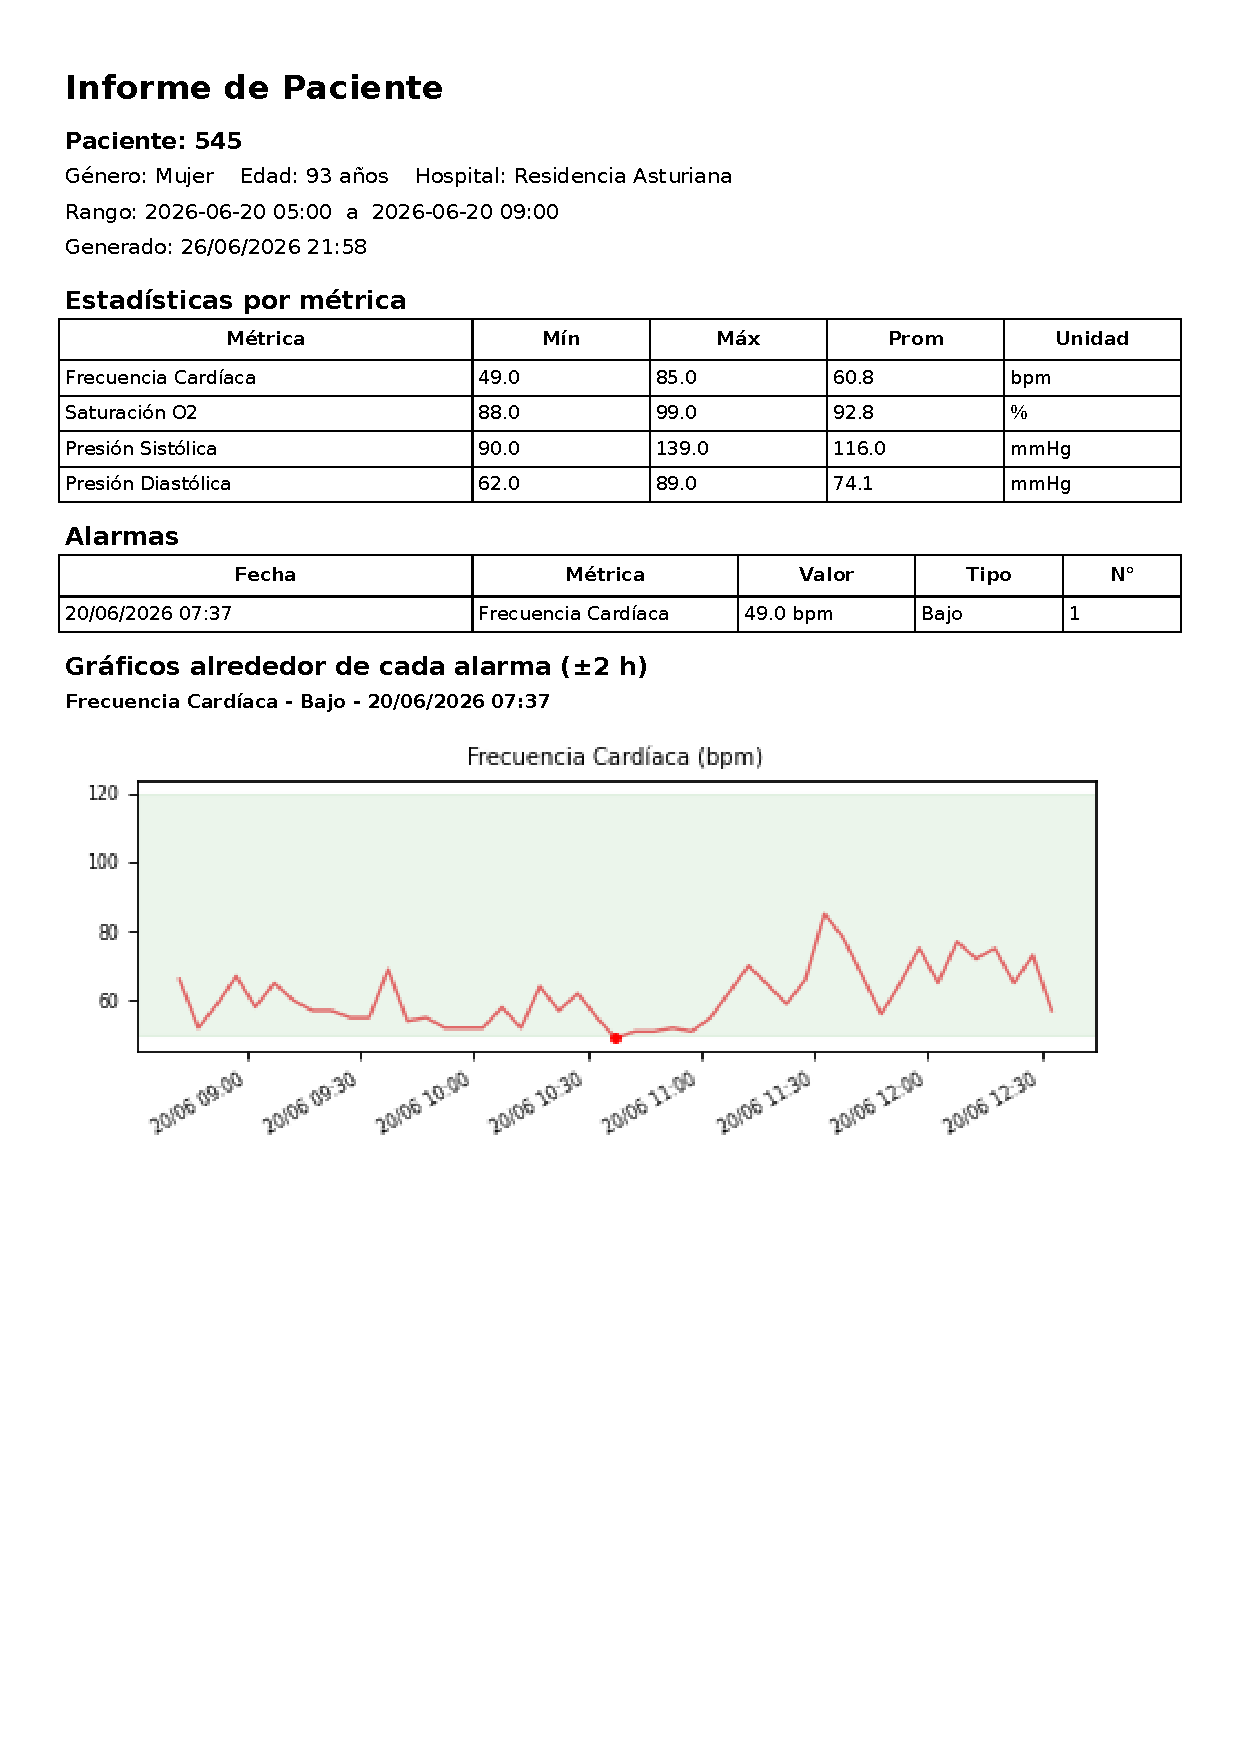
\includepdf[pages=-,pagecommand={\thispagestyle{plain}}]{./reportes/informe_alarma.pdf}

\clearpage
\subsection*{Anexo B. Respuestas a la evaluación de usabilidad}

Se incluyen las respuestas completas de las dos participantes a la evaluación de
usabilidad descrita en el Capítulo~7 —el guion de tareas, la escala SUS y las
preguntas abiertas—.

\medskip
\noindent\textbf{Médica de la Residencia Asturiana.}

\begin{center}
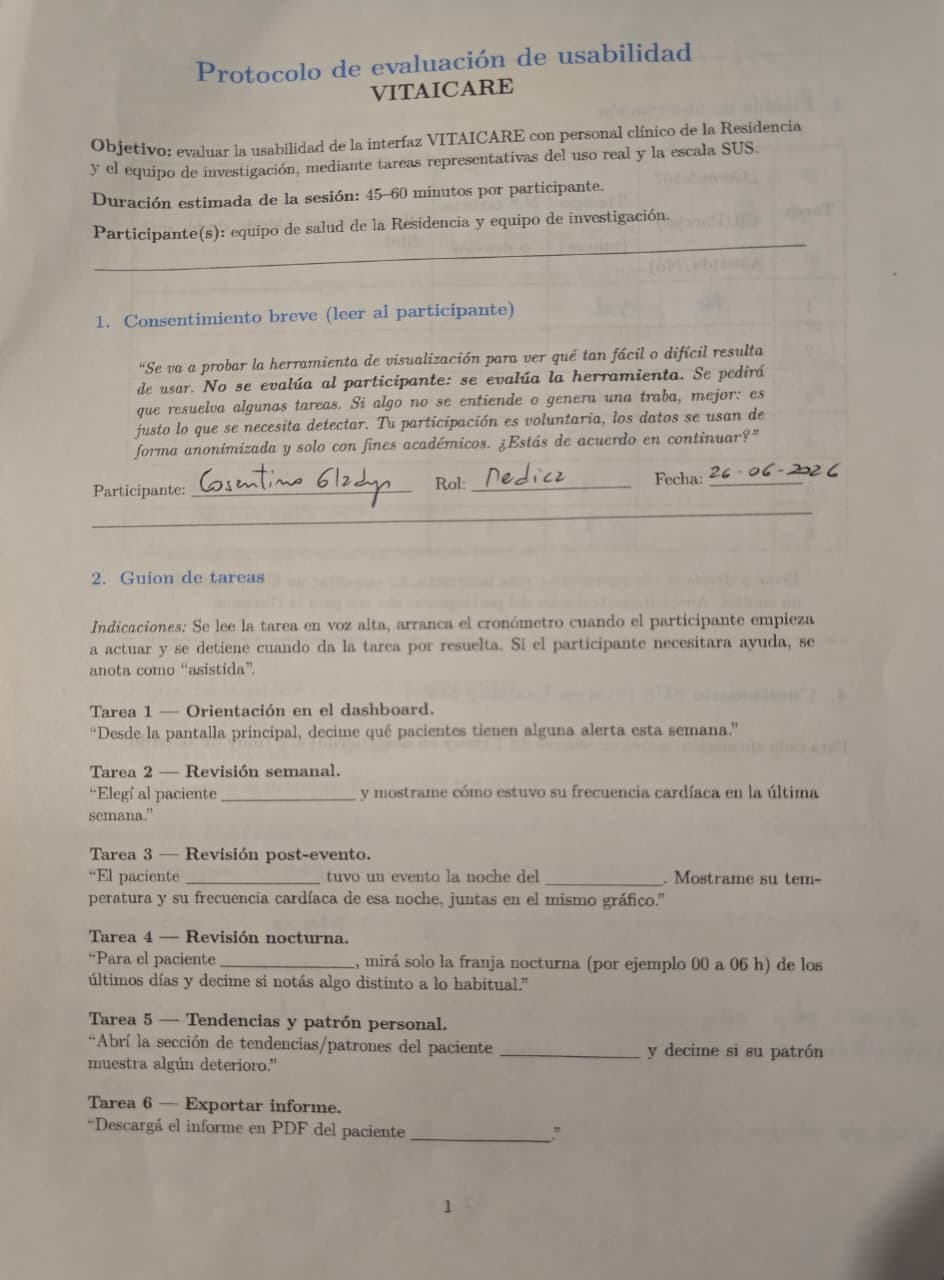
\includegraphics[width=0.82\textwidth]{./respuestas_usabilidad/g1.jpeg}\par\medskip
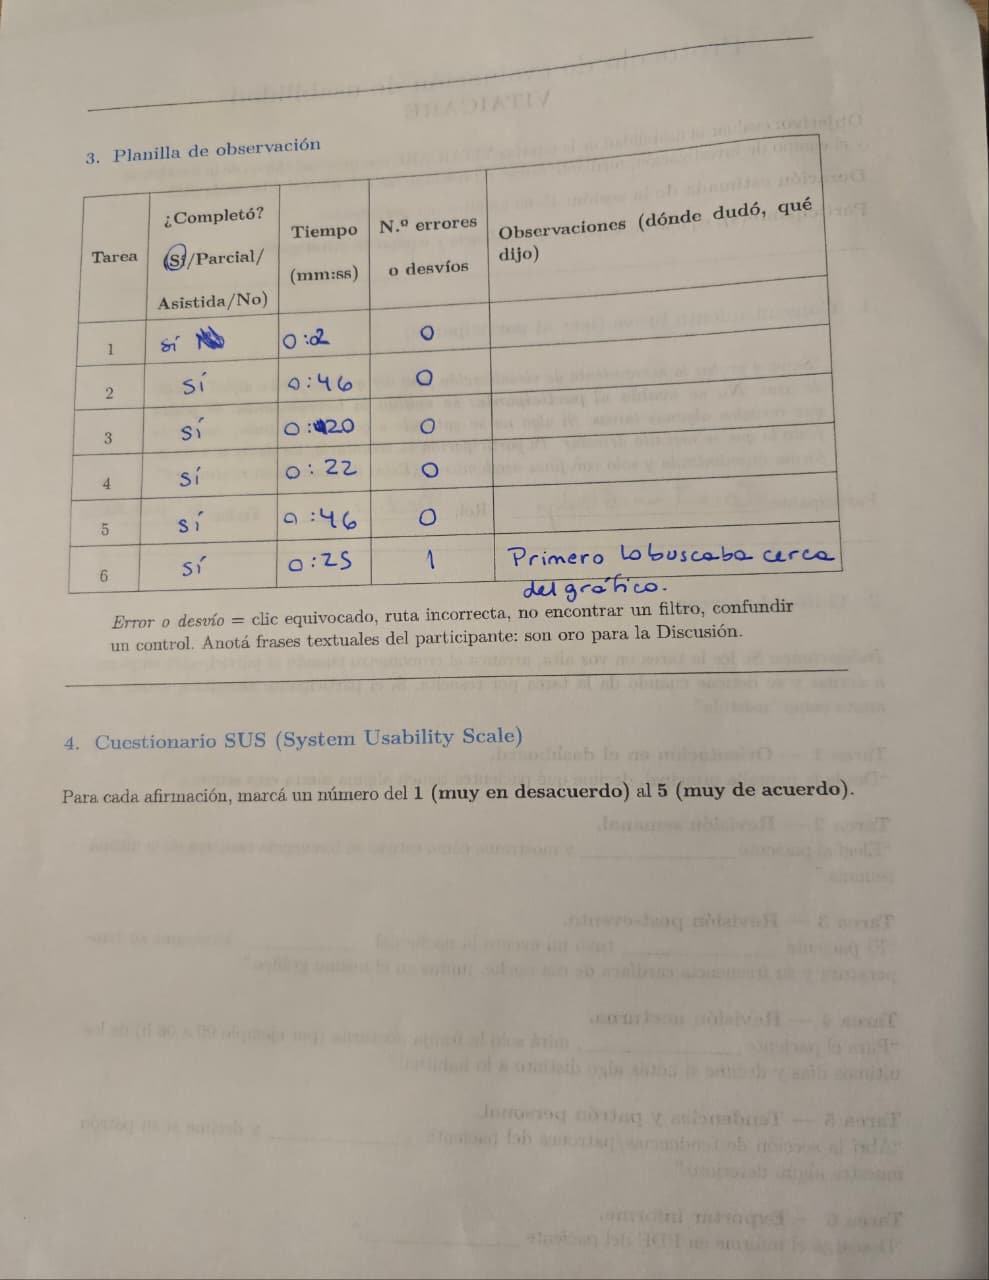
\includegraphics[width=0.82\textwidth]{./respuestas_usabilidad/g2.jpeg}\par\medskip
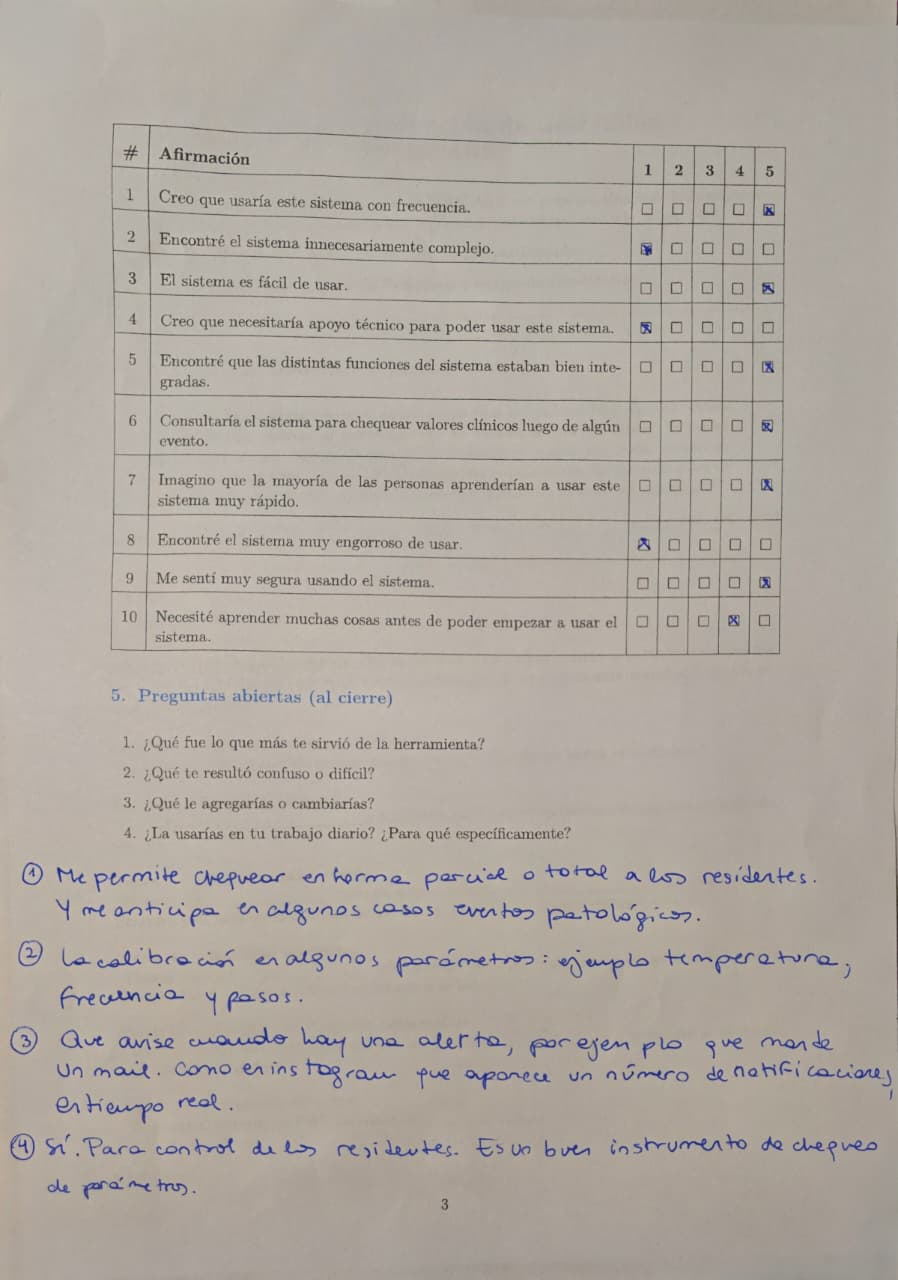
\includegraphics[width=0.82\textwidth]{./respuestas_usabilidad/g3.jpeg}
\end{center}

\clearpage
\noindent\textbf{Investigadora 1 (Universidad de Alcalá).}

\begin{center}
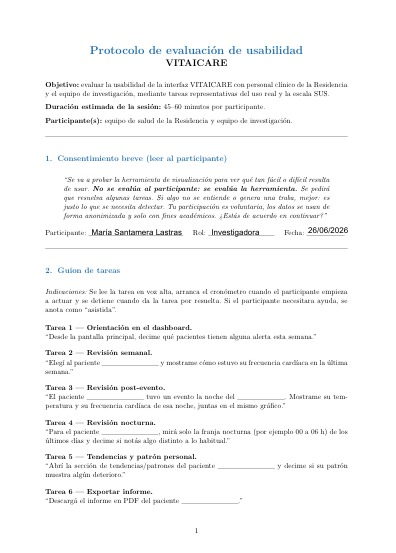
\includegraphics[width=0.82\textwidth]{./respuestas_usabilidad/m1.jpeg}\par\medskip
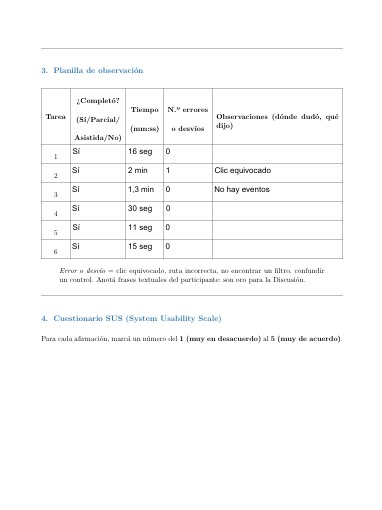
\includegraphics[width=0.82\textwidth]{./respuestas_usabilidad/m2.jpeg}\par\medskip
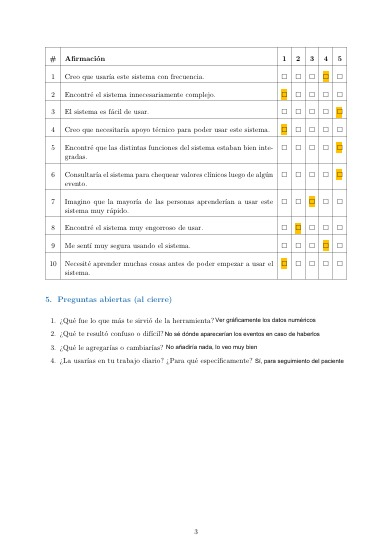
\includegraphics[width=0.82\textwidth]{./respuestas_usabilidad/m3.jpeg}
\end{center}

\clearpage
\noindent\textbf{Investigadora 2 (Universidad de Alcalá).}

\begin{center}
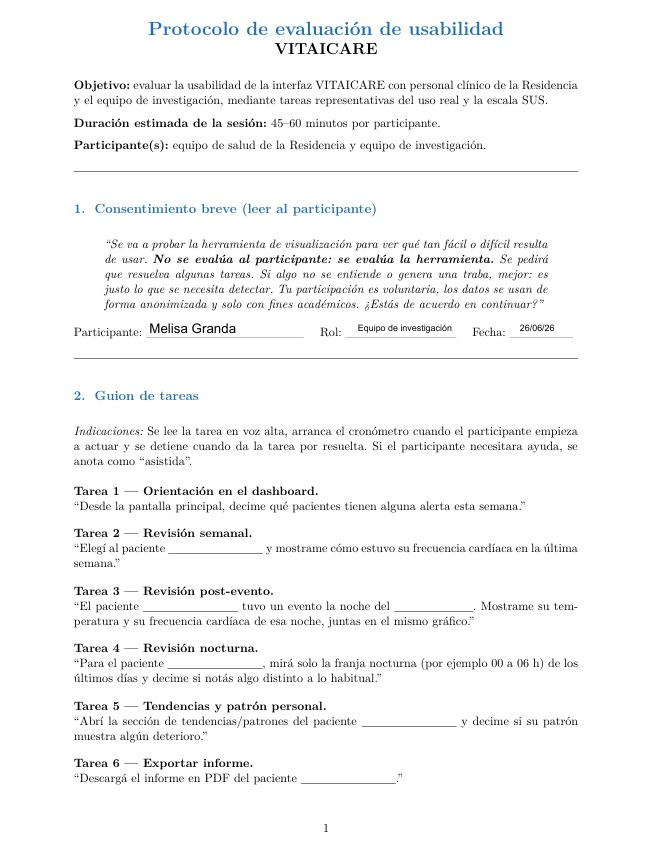
\includegraphics[width=0.82\textwidth]{./respuestas_usabilidad/meli1.jpeg}\par\medskip
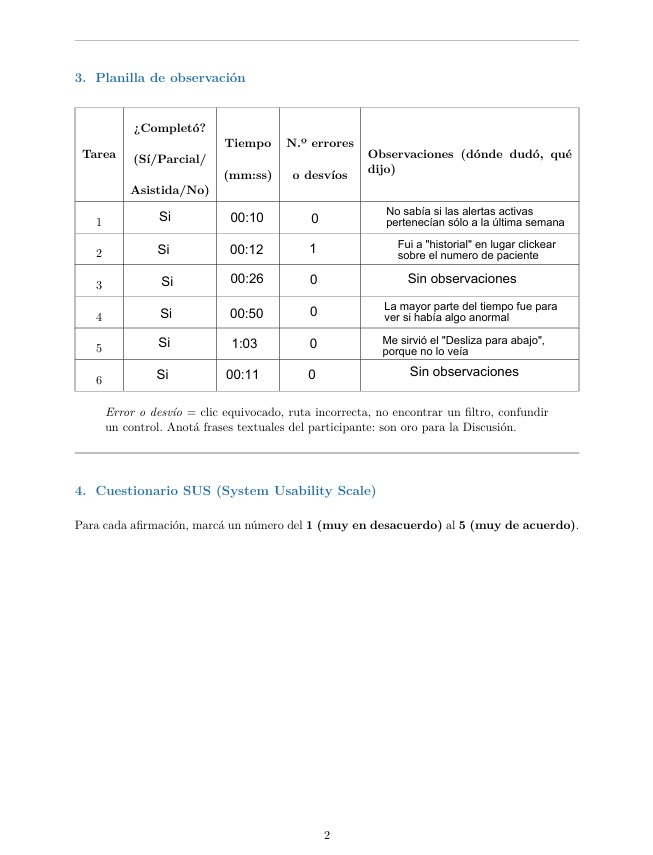
\includegraphics[width=0.82\textwidth]{./respuestas_usabilidad/meli2.jpeg}\par\medskip
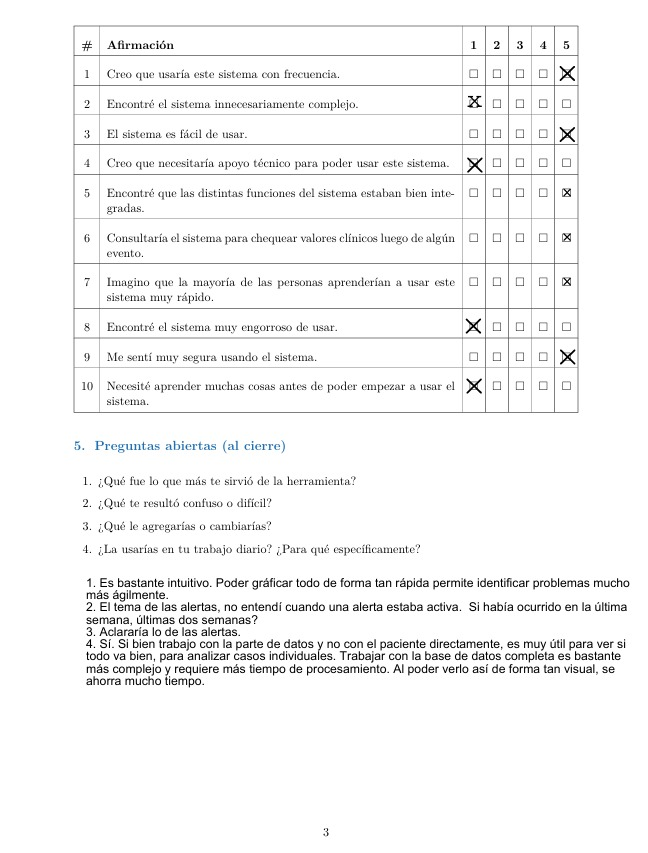
\includegraphics[width=0.82\textwidth]{./respuestas_usabilidad/meli3.jpeg}
\end{center}

\clearpage
\noindent\textbf{Tutor del proyecto (Instituto Tecnológico de Buenos Aires).}

\begin{center}
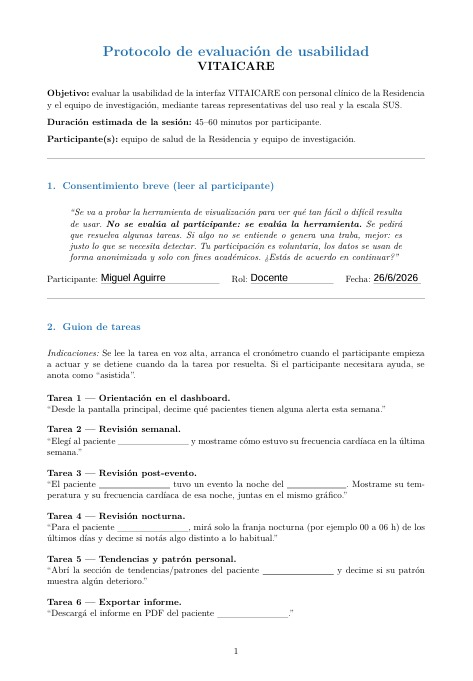
\includegraphics[width=0.82\textwidth]{./respuestas_usabilidad/mi1.jpeg}\par\medskip
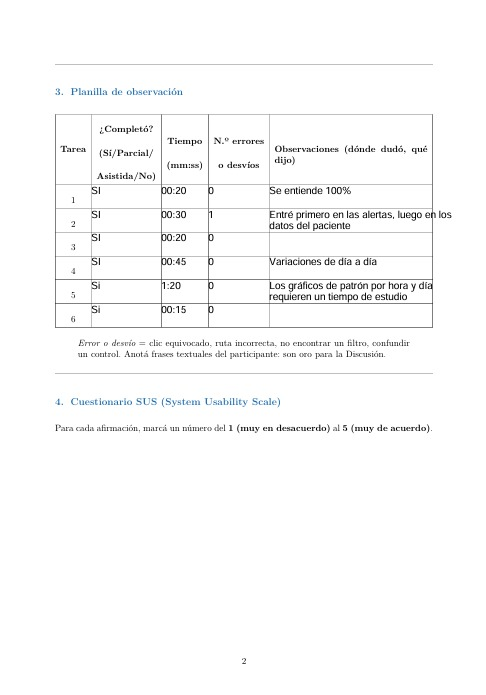
\includegraphics[width=0.82\textwidth]{./respuestas_usabilidad/mi2.jpeg}\par\medskip
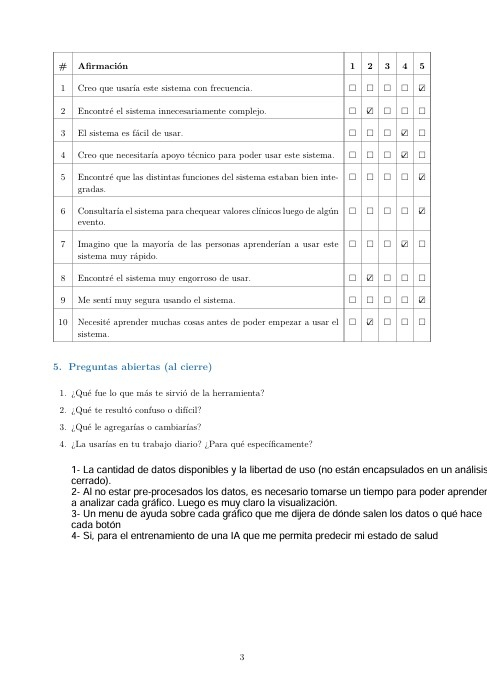
\includegraphics[width=0.82\textwidth]{./respuestas_usabilidad/mi3.jpeg}
\end{center}

\end{document}
